\documentclass[a4paper,11pt,titlepage,twoside,openany]{book}

\usepackage{natbib}
\usepackage{setspace} \onehalfspacing
\usepackage{parskip}

% \newcommand{\only}{title}

\include{paper}
%include paper.fmt


% add horizontal lines above and below figures
\let\oldfigure\figure\let\oldendfigure\endfigure
\let\oldtable\table\let\oldendtable\endtable
\let\oldcaption\caption
\newcommand{\newcaption}[1]{\hrule\oldcaption{#1}}
\renewenvironment{figure}
    {\let\caption\newcaption\oldfigure\hrule}
    {\let\caption\oldcaption\oldendfigure}
\renewenvironment{table}
    {\let\caption\newcaption\oldtable\hrule}
    {\let\caption\oldcaption\oldendtable}

% simplify rules
\newenvironment{simplify}
    {\bigskip\begin{tabular*}{\linewidth}{@@{}p{10cm}@@{\extracolsep{\fill}}r}}
    {\end{tabular*}}
\newcommand{\simp}[2]{\vspace{-7mm} #2 & (#1) \\[-5mm]}

% margins
\addtolength{\topmargin}{-5mm}
\addtolength{\textheight}{10mm}

\newenvironment{console}
    {\begin{singlespace}\sf}
    {\end{singlespace}}


\begin{document}

%include paper.fmt

\title{Transformation and Analysis \\ of Functional Programs}
\author{Neil Mitchell}
\date{\normalsize{
    \vspace{20mm}
    Submitted for the degree of Doctor of Philosophy \\
    \vspace{10mm}
    Department of Computer Science \\
    University of York \\
    \today}}

\maketitle

\setcounter{page}{2}

\chapter*{Abstract}

This thesis deals with the transformation and analysis of functional programs. We show how to make functional programs shorter, faster and safer. Throughout, we work on a core lazy functional language, to which Haskell programs can be reduced. We present examples, develop prototype tools and show detailed results for sample program.

We make programs \textit{shorter} by defining a library which abstracts over common data traversal patterns, removing \textit{boilerplate} code. Our library restricts traversals to have value-specific behaviour for just one type, allowing a simpler programming model. Our library allows concise expression of traversals with competitive performance.

We make programs \textit{faster} by applying a variant of \textit{supercompilation} to core programs. We have implemented a supercompiler, and test it using standard Haskell benchmarks. As a result of our practical experiments, we have identified modifications to the standard supercompilation techniques -- particularly with respect to let bindings and the generalisation technique.

We make programs \textit{safer} by automatically checking for potential pattern-match errors. We define a transformation that takes a higher-order program and produces an equivalent program with fewer functional values, typically a first-order program. We then define an analysis on a first-order language which checks statically that, despite the possible use of partial (or non-exhaustive) pattern matching, no pattern-match failure can occur.


\tableofcontents
\listoffigures
\listoftables

\chapter*{Acknowledgements}

Throughout the PhD I have been supported by an EPSRC PhD studentship. I would like to thank Colin Runciman, who has supervised me for the last 6 years. Colin taught me functional programming in the first place, has helped me with technical problems, and in particular has helped me to express myself more clearly using the written word. In addition to Colin's supervision, all the members of the PLASMA group have provided interesting discussions, lots of technical debate and answers to \LaTeX\ problems.

Many people in the Haskell community have made technical contributions, of both ideas and code, have encouraged my progress, and have answered my questions. Included in this list are Bj\"{o}rn Bringert, Brandon Moore, Damien Sereni, Duncan Coutts, Eric Mertens, J\"{u}rgen Doser, Jules Bean, Koen Claessen, Matthew Danish, Peter Jonsson, Simon Marlow, Simon Peyton Jones, Stefan O'Rear, Tim Chevalier and the whole of the Haskell community, particularly \verb"#haskell". The vast number of people who have helped ensures that I have certainly forgotten many people.

While doing a PhD, I have appreciated the presence of many friends -- including all the members of the York University Karate Club, and the many residents of 232 Melrosegate. Lastly, thanks to my parents, who have given me the freedom to make my own decisions, and an occasional email to check on my wellbeing.

\chapter*{Declaration}

Chapter \ref{chp:background} has some overlap with material published in \cite{me:yhc_core}. Chapter \ref{chp:uniplate} is based on the paper \cite{me:uniplate}, which appeared at the Haskell Workshop 2007. Chapter \ref{chp:supero} is based on the paper \cite{me:supero_ifl} which was presented at IFL 2007, and the revised paper \cite{me:supero} which has been accepted into the post proceedings. Chapter \ref{chp:firstify} is based on the paper \cite{me:firstify_icfp} which has been submitted to ICFP 2008. Chapter \ref{chp:catch} follows on from the original papers \cite{me:catch_tfp_original,me:catch_tfp} presented at TFP 2005 and appearing in the post proceedings, and is based on the paper \cite{me:catch_icfp} submitted to ICFP 2008.

Expect for the above cases and where stated, all of the work contained within this thesis represents the original contribution of the author.

%include paper.fmt

\chapter{Introduction}

This thesis contributes to the field of functional programming. In particular, we have worked with the lazy functional language Haskell \cite{haskell}. The Haskell language is pure, requiring side effects to be specifically annotated and sequenced. Often Haskell programs can be regarded as high-level specifications of a problem. While we have implemented all our techniques in Haskell, most of them should be applicable to any functional language. We first discuss our motivation for the problems we have tackled, then the implementations available, followed by a review of the following chapters.

\section{Motivation and Objectives}

Mention the names of the tools in here.

Haskell is a strongly typed language, ensuring that a large class of errors are caught at compile time. The strong typing has lead people to state that ``if a Haskell program type checks, it usually works''. However, despite all the guarantees that the type system gives, the expression |head []| will crash at runtime. The initial motivation for this thesis was the elimination of such errors.

A Haskell program may fail in one of three ways: (1) it calls |error|; (2) it non-terminates; (3) it performs the wrong computation. Of these, the first two are easily stated as general properties of all programs, while the final one requires program specific annotations. We have focused on the route requiring no additional annotations. We have decided to check for calls to |error|. Termination checking has been investigated thoroughly, both in general term-rewriting systems and in Haskell, so we chose to go for |error| calls. We also feel that in practical programs, the issue of pattern-match errors occurs more frequently than non-termination. Also, if a checker falsely claims that a program has a pattern-match error, it can usually be worked around.

We first developed the Catch checker for a first-order language. We then attempted to extend the checker to a higher-order language, but failed. A higher-order program hides the flow control within a program, and requires functions to be annotated with information about pattern-safety in complex ways. As a result we looked at the alternative, making a higher-order program first-order. We started by taking existing transformations, particularly specialisation, and combining them into a complete defunctionalisation method.

After making a program first-order, it tends to execute faster than before. As we explored this side-effect of the defunctionalisation, we were drawn in new directions -- particularly supercompilation. The idea was that you could obtain a defunctionalisation method by taking a very powerful program optimiser, and restricting it. We started with the work on supercompilation. Unfortunately, this hope turned out to be ill-founded. Supercompilation is not a suitable vehicle for defunctionalisation. However, we were able to push our original defunctionalisation method, using techniques inspired by supercompilation, into a usable transformation. The defunctionalisation method is primarily designed as a transformation before analysis, particularly for our pattern-match analyser.

Having started upon a supercompiler, we decided to finish. Our initial goal within the pattern-match checker was to require no annotations, and we developed our supercompiler along the same lines. While other Haskell compilers make use of knowledge about type classes, and hand-written deforestation rules, we assume no knowledge about the underlying program. Our hope is that freeing people from annotating their code will allow a more unrestricted expression of ideas, discouraging people from thinking about the performance.

Our final contribution is the Uniplate library. The expression type of the Core language we work with has over ten constructors. Most of these constructors typically contain embedded subexpressions. For most operations, we wish to have value-specific behaviour for a handful of constructor, but some default operation for all the others. We started developing a small collection of useful functions to deal with this complexity, and gradually abstracted the ideas. After a while, the Uniplate library had appeared in its current form. The Uniplate library stands apart from the rest of the thesis in that it does not work on a core functional language, but is instead a general purpose library. However, the Uniplate techniques have been invaluable in implementing the other transformations.


\section{Implementations}

We have implemented all the ideas presented in this thesis, and include sample code in the appropriate chapters. We used a monadic framework to deal with issues such as obtaining unique free variables and tracking termination constraints. But to simplify the presentation, we ignore these issues -- they are mostly tedious engineering concerns, and do not effect the underlying algorithm.

All the code is available from the authors homepage\footnote{\url{http://www.cs.york.ac.uk/~ndm/}}. Additionally, we have released a number of programs on the Hackage website\footnote{\url{http://hackage.haskell.org/}}. In particular, the following packages correspond to the following parts of the thesis. We have also listed the dependencies between packages.

\begin{description}
\item[homeomorphic] This is a library for homeomorphic embedding, as described in \S\ref{sec:homeomorphic}.
\item[yhccore] This is a library providing the data type for Yhc's Core language. Requires uniplate.
\item[uniplate] This is the library described in Chapter \ref{chp:uniplate}.
\item[supero] This is the program described in Chapter \ref{chp:supero}. Requires yhccore, homeomorphic and uniplate.
\item[firstify] This is the library described in Chapter \ref{chp:firstify}. Requires yhccore, homeomorphic and uniplate.
\item[catch] This is the program described in Chapter \ref{chp:catch}. Requires yhccore, homeomorphic, uniplate and firstify.
\end{description}

\section{Chapter Outline}

The Background chapter (\ref{chp:background}) covers the background material needed by the following chapters. The main focus is on a common Core language which is used in the subsequent sections. Additionally, it covers the homeomorphic embedding, a relation used to ensure termination in a number of situations.

The Boilerplate Removal chapter (\ref{chp:uniplate}) describes the Uniplate library. In particular, it describes the interface to the library -- both the traversal functions and the information a type must provide. It also compares the Uniplate library to the Scrap Your Boilerplate (SYB) library, and the Compos library -- both for speed and conciseness.

The Supercompilation chapter (\ref{chp:supero}) describes the design and implementation of the Supero tool. The method includes new steps for generalisation and new techniques to deal with let bindings. The results shown that it is possible to obtain a speedup, even when compared to a mature optimising compiler such as GHC.

The Defunctionalisation chapter (\ref{chp:firstify}) describes how to combine several existing transformations to produce a defunctionalisation method. The primary contribution is how to restrict the existing methods to ensure they terminate and cooperate well to obtain a program with few residual functional values. Results are presented for some of the nofib suite, showing that usually a program can be made first-order.

The Pattern Match Analysis chapter (\ref{chp:catch}) describes the implementation of the Catch tool. In particular, it presents a mechanism for reasoning about programs using a constraint language. Two constraint languages are introduced, which are compared. Finally, results are presented for the nofib suite, and for several larger programs.

The Conclusions and Relation Work chapter (\ref{chp:conclusions}) gives directions for future work, and makes concluding remarks.


%include thesis.fmt

\hsdef{\begin{comment}
a,e,v_i,x_i,i,f
Ord,letrec,xs,bottom
\end{comment}}
\begin{comment}
\begin{code}
import Prelude hiding (repeat)
import Data.List hiding (repeat)

data Expr = EVar String
          | ECon String [Expr]
          | EFun String [Expr]
          | EApp Expr [Expr]
          | ELam String Expr
          | ELet String Expr Expr
          | ECase Expr [Alt]

data Alt = EAlt String [String] Expr

unions = foldr1 union

expensive = undefined
dummy = ()
\end{code}
\end{comment}

\chapter{Background}
\label{chp:background}

In this chapter we introduce the background material and general notations used throughout the rest of this thesis. We start by introducing a Core language in \S\ref{secB:core}, then discuss its sharing properties in \S\ref{secB:sharing} and how we generate Core in \S\ref{secB:generating_core}. We then cover the homeomorphic embedding relation in \S\ref{secB:homeomorphic}, particularly applied to the expression type of our Core language.

\section{Core Language}
\label{secB:core}

\begin{figure}
\renewcommand{\f}[1]{\text{\hspace{1cm}#1}}
\ignore\begin{code}
prog  ::=  fs_                 {-"\f{program}"-}

func  ::=  f vs_ = x           {-"\f{function}"-}

expr  ::=  v                   {-"\f{variable}"-}
      |    c xs_               {-"\f{constructor application}"-}
      |    f xs_               {-"\f{function application}"-}
      |    x xs_               {-"\f{general application}"-}
      |    \v -> x             {-"\f{lambda abstraction}"-}
      |    let v = x in y      {-"\f{let binding, non-recursive}"-}
      |    case x of as_       {-"\f{case expression}"-}

alt   ::=  c vs_ -> x          {-"\f{case alternative}"-}
\end{code}

Where |v| ranges over variables, |c| ranges over constructors, |f| ranges over function names, |x| and |y| range over expressions and |a| ranges over case alternatives. \\
\caption{Syntax for the Core language.}
\label{figB:core}
\end{figure}

\todo{Mention the semantics of Core, possibly with a reference to the semantics/definition of Haskell}

\todo{Explain the duplication present in the language}

The syntax of our Core language is given in Figure \ref{figB:core}. To specify a list of items of unspecified length we write either \ignore|x_1,...,x_n| or |xs_|. Our Core language is higher order and lazy, but lacks much of the syntactic sugar found in Haskell. In later chapters it will be necessary to make a distinction between higher-order and first-order programs, so our Core language has some redundancy in its representation. The language is based upon Yhc.Core, a semantics for which is given in \cite{me:yhc_core}.

A program is a list of functions, with a root function named |main|. A function definition gives a name, a list of arguments and a body expression. Variables and lambda abstractions are much as they would be in any Core language.  Pattern matching occurs only in case expressions; alternatives match only the top level constructor and are exhaustive, including an |error| alternative if necessary. We have three forms of application, all of which take two values: the first value may be either a constructor, a top-level named function, or any arbitrary expression; the second value is a list of arguments, which may be empty. These forms of application give rise to three equivalences:

\ignore\begin{code}
(x xs_) ys_ == x xs_ ys_
(f xs_) ys_ == f xs_ ys_
(c xs_) ys_ == c xs_ ys_
\end{code}

We allow a list of variables to appear in a lambda abstraction and a list of bindings to appear in a let. This syntactic sugar can be translated away using the following rules:

\ignore\begin{code}
\v vs_ -> x              => \v -> (\vs_ -> x)
let v = x ; binds_ in y  => let v = x in (let binds_ in y)
let v vs_ = x xs_ in y   => let v = x in (let vs_ = xs_ in y)
\end{code}

The arity of a top-level function is the number of arguments in its associated definition. In any application, if the function is given fewer arguments than its arity we refer to it as \textit{partially-applied}, matching the arity is \textit{fully-applied}, and more than the arity is \textit{over-applied}.

Some functions are used but lack corresponding definitions in the program. These are defined to be \textit{primitive}. They have some meaning to an underlying runtime system, but are not available for transformation. A primitive function may perform an action such as outputting a character to the screen, or may manipulate primitive numbers such as addition.

The largest difference between our Core language and GHC-Core \cite{ghc_core} is that our Core language is untyped. The Core is generated from well-typed Haskell, and is guaranteed not to fail with a type error. All our algorithms could be implemented equally well in a typed Core language, but we prefer to work in an untyped language for simplicity of implementation. For describing data types we use the same notation as Haskell 98. One of the most common data types is the list, which can be defined as:

\begin{code}
data List alpha = Nil | Cons alpha (List alpha)
\end{code}

A list is either an empty list, or a cons cell which contains an element of the list type and the tail of the list. For example the list of 1,2,3 would be written |(Cons 1 (Cons 2 (Cons 3 Nil)))|. We allow the syntactic sugar of representing |Cons| as a right-associative infix application of |(:)| and |Nil| as |[]| -- allowing us to write |(1:2:3:[])|. We also permit |[1,2,3]|.


\subsection{Operations on Core}

There are several operations that can be defined on our Core expressions type. We present some of those used in later chapters.

\subsubsection{General Operations}

\begin{figure}
\begin{code}
type CtorName  = String
type VarName   = String
type FuncName  = String

body   :: FuncName  -> Expr
args   :: FuncName  -> [VarName]
rhs    :: Alt       -> Expr
arity  :: String    -> Int
ctors  :: CtorName  -> [CtorName]
\end{code}
\caption{Operations on Core.}
\label{figB:core_operations}
\end{figure}

Figure \ref{figB:core_operations} gives the signatures for helper functions over the core data types. We use the functions |body f| and |args f| to denote the body and arguments of the function definition |f|. We use the function |rhs| to extract the expression on the right of a case alternative. Every function and constructor has an arity, which can be obtained with the |arity| function. To determine alternative constructors the |ctors| function can be used; for example \h{stmt}|ctors "True" = ["False", "True"]| and \h{stmt}|ctors "[]" = ["[]",":"]|.


\subsubsection{Substitution}

We define \ignore|e[v / x]| to be the capture-free substitution of the variable |v| for the expression |x| within the expression |e|. We define \ignore|e[v_1,...,v_n / x_1,...,x_n]| to be the simultaneous substitution of each variable |v_i| for each expression |x_i| in |e|.

\begin{example}
\ignore\begin{code}
(v + 1)[v / 2]               => 2 + 1
(let v = 3 in v + 1)[v / 2]  => let v = 3 in v + 1
\end{code}
\end{example}

\subsubsection{Variable Classification}

\begin{figure}
\begin{code}
freeVars :: Expr -> [VarName]
freeVars (EVar v       ) = [v]
freeVars (ECon c xs_   ) = freeVars' xs_
freeVars (EFun f xs_   ) = freeVars' xs_
freeVars (EApp x xs_   ) = freeVars x `union` freeVars' xs_
freeVars (ELam v x     ) = freeVars x \\ [v]
freeVars (ELet v x y   ) = freeVars x `union` (freeVars y \\ [v])
freeVars (ECase x as_  ) = freeVars x `union` unions (map f as_)
    where f (EAlt c vs_ y) = freeVars y \\ vs_

freeVars' xs_ = unions (map freeVars xs_)
\end{code}
\caption{Free variables of an expression.}
\label{figB:free_variables}
\end{figure}

An occurrence of a variable |v| is \textit{bound} in |x| if it occurs on the right-hand side a case alternative whose pattern includes |v|, as the argument of an enclosing lambda abstraction or as a binding in an enclosing let expression; all other variables are \textit{free}. The set of free variables of an expression |e| is denoted by |freeVars e|, and can be computed using the function in Figure \ref{figB:free_variables}.

In order to avoid accidental variable name clashes while performing transformations, we demand that all variables within a program are unique. All transformations may assume and should preserve this invariant.

\subsection{Simplification Rules}
\label{secB:core_simplify}

\begin{figure}
\begin{simplify}
\simp{app-app}{
\ignore\begin{code}
(x xs_) ys_
    => x xs_ ys_
\end{code}}

\simp{fun-app}{
\ignore\begin{code}
(f xs_) ys_
    => f xs_ ys_
\end{code}}

\simp{con-app}{
\ignore\begin{code}
(c xs_) ys_
    => c xs_ ys_
\end{code}}

\simp{case-con}{
\ignore\begin{code}
case c xs_ of {... ; c vs_ -> y ; ...}
    => let vs_ = xs_ in y
\end{code}}

\simp{lam-app}{
\ignore\begin{code}
(\v -> x) y
    => let v = y in x
\end{code}}

\simp{case-app}{
\ignore\begin{code}
(case x of {c_1 vs__1 -> y_1 ; ... ; c_n vs__n -> y_n}) z
    => case x of {c_1 vs__1 -> y_1 z ; ... ; c_n vs__n -> y_n z}
\end{code}}

\simp{let-app}{
\ignore\begin{code}
(let v = x in y) z
    => let v = x in y z
\end{code}}

\simp{let-case}{
\ignore\begin{code}
let v = x in (case y of {c_1 vs__1 -> y_1 ; ... ; c_n vs__n -> y_n})
    => case y of  {  c_1 vs__1  -> let v = x in y_1
                  ;  ...
                  ;  c_n vs__n  -> let v = x in y_n}
    where v {-" \hbox{is not used in } "-} y
\end{code}}

\simp{case-let}{
\ignore\begin{code}
case (let v = x in y) of as_
    => let v = x in (case y of as_)
\end{code}}

\simp{case-case}{
\ignore\begin{code}
case (case x of {c_1 vs__1 -> y_1 ; ... ; c_n vs__n -> y_n}) of as_
    => case x of  {  c_1 vs__1  -> case y_1 of as_
                  ;  ...
                  ;  c_n vs__n  -> case y_n of as_ }
\end{code}}

\simp{case-lam}{
\ignore\begin{code}
case x of {... ; c vs_ -> \v -> y ; ...}
    => \z -> case  x of
                   {... z ; c vs_ -> (\v -> y) z ; ... z}
\end{code}}

\simp{let}{
\ignore\begin{code}
let v = x in y
    => y[v/x]
    where x {-" \hbox{is used once in } "-} y
\end{code}}
\end{simplify}
\caption{Simplification rules.}
\label{figB:simplify}
\end{figure}

\todo{State that the rules duplicate code, but not work Conjecture the are confluent, if I believe it to be true}

We present several simplification rules in Figure \ref{figB:simplify}, which can be applied to our Core language. These rules are standard and would be applied by any optimising compiler \cite{spj:transformation}. All the rules preserve both the semantics and the sharing behaviour of an expression.

The (app-app), (fun-app) and (con-app) rules normalise applications. The (case-con) and (lam-app) rules simply follow the semantics, using let expressions to preserve the sharing. The (case-app), (let-case) and (case-case) rules move outer expressions over an inner case expression, duplicating the outer expression in each alternative. The (case-lam) rule promotes a lambda from inside a case alternative outwards. The (let-app) and (let-case) rules move an expression over an inner let expression. The (let) rule substitutes let expressions where the bound variable is used only once, and therefore no loss of sharing is possible.


\begin{comment}
\section{Semantics}
\label{secB:semantics}

The evaluation strategy of our Core language is lazy. We specify a reduction to weak-head normal form (WHNF) in Figure \ref{figB:whnf} and a reduction to normal form (NF) in \ref{figB:nf}. We have assumed that all applications are translated to general applications where the second value is a 1-element list. The \ignore|_F| function translates a function name to an associate expression incorporating the program arguments as variables in a lambda, and the body as the body of that lambda. The grammar for expressions in WHNF is:

\ignore\begin{code}
r  =  c \< xs_ \>  {-" \text{  constructor} "-}
   |  \v -> x      {-" \text{  lambda} "-}
   |  bottom       {-" \text{  bottom/undefined} "-}
\end{code}

The grammar for expression in NF is:

\ignore\begin{code}
n  =  c \< ns_ \>  {-" \text{  constructor} "-}
   |  \v -> x      {-" \text{  lambda} "-}
   |  bottom       {-" \text{  bottom/undefined} "-}
\end{code}

\newcommand{\sem}[1]
    {& \begin{array}{c}#1\smallskip\end{array}}
\newcommand{\semm}[2]
    {& \frac{\begin{array}{c}#1\end{array}}
            {\begin{array}{c}#2\smallskip\end{array}}}
\newcommand{\semmm}[3]
    {& \frac{\begin{array}{c}#1\\#2\end{array}}
            {\begin{array}{c}#3\smallskip\end{array}}}

\begin{figure}
\begin{eqnarray}
\sem
    {\ignore|c => c \< \>|}
\\ \semmm
    {\ignore|_F(f) = x|}
    {\ignore|x => r|}
    {\ignore|f => r|}
\\ \semm
    {\ignore|x => bottom|}
    {\ignore|x y => bottom|}
\\ \semm
    {\ignore|x => c \< xs_ \>|}
    {\ignore|x y => c \< xs_ y \>|}
\\ \semmm
    {\ignore|x => \v -> x'|}
    {\ignore|x'[v/y] => r|}
    {\ignore|x y => r|}
\\ \semm
    {\ignore|y[v/x] => r|}
    {\ignore|let v = x in y => r|}
\\ \semmm
    {\ignore|x => c \< xs_ \>|}
    {\ignore|y[vs_ / xs_] => r|}
    {\ignore|case x of {... ; c vs_ -> y ; ...} => r|}
\\ \semm
    {\ignore|x => bottom|}
    {\ignore|case x of alts_ => bottom|}
\end{eqnarray}
\caption{Reduction to weak-head normal form, |(=>)|.}
\label{figB:whnf}
\end{figure}

\begin{figure}
\begin{eqnarray}
\semm
    {\ignore|x => bottom|}
    {\ignore|x =>* bottom|}
\\ \semm
    {\ignore|x => \v -> y|}
    {\ignore|x =>* \v -> y|}
\\ \semmm
    {\ignore|x => c \< xs_ \>|}
    {\ignore|xs_ =>* xs_' |}
    {\ignore|x =>* c \< xs_' \>|}
\end{eqnarray}
\caption{Reduction to normal form, \ignore|(=>*)|.}
\label{figB:nf}
\end{figure}

Our semantics does not respect sharing, this topic is dealt with in \S\ref{secB:sharing}. The evaluation of a program corresponds to reducing |main| to NF.

We never descend below a bound variable without replacing that variable, therefore any remaining variable would have to be free in the definition of the program, which is not permitted. Consequently, there is no rule for a variable. We choose not evaluate inside a lambda, even on \ignore|=>*|, as this would generate a free variable. The \ignore|_F| mapping never crashes, as it is checked statically that all mentioned function names exist in the mapping.

The only way an undefined value may be initially generated is by a call to the error function in the program, i.e. \ignore|_F(error) = \v -> bottom|. If a computation forces a |bottom| value, in the scrutinee of a case or the first argument of an application, the |bottom| is propagated.

There is no rule for case of a lambda abstraction, as this situation is not permitted by the type system. Similarly, the type system plus the exhaustiveness of case branches means that if the scrutinee successfully evaluates, it will match exactly one alternative.
\end{comment}


\section{Sharing}
\label{secB:sharing}

This section informally discusses the relevant sharing properties of Haskell. In general, any optimisation must take account of sharing, but semantic analysis can sometimes ignore the effects of sharing. The sharing present in Haskell is not specified in the Haskell Report \cite{haskell}, but a possible interpretation is defined elsewhere \cite{bakewell:space_semantics}.

\subsection{Let bindings}

A let expression introduces \textit{sharing} of the computational result of expressions. Consider the expression:

\begin{example}
\ignore\begin{code}
let x = f 1
in x + x
\end{code}

The semantic rules for evaluating this expression result in:

\ignore\begin{code}
(x + x)[x / f 1]
(f 1 + f 1)
\end{code}

In the semantics, the expression |f 1| is reduced twice. However, the a compiler would only evaluate |f 1| once. The first time the value of |x| is demanded, |f 1| evaluates to WHNF, and is bound to |x|. Any successive examinations of |x| return immediately, pointing at the same result.
\end{example}

\todo{Fix the bug concerning linearity and lambdas, REQUIRED. Consider let x = expensive in (let f  = \y -> x + y in map f xs))}

\begin{figure}
\begin{code}
occurs :: VarName -> Expr -> Int
occurs v (EVar v'      ) = if v == v' then 1 else 0
occurs v (ECon c xs_   ) = occurss v xs_
occurs v (EFun f xs_   ) = occurss v xs_
occurs v (EApp x xs_   ) = occurss v (x:xs_)
occurs v (ELam v' x    ) = if v == v' then 0 else occurs v x
occurs v (ELet v' x y  ) = if v == v' then 0 else occurss v [x,y]
occurs v (ECase x as_  ) = occurs v x + maximum (map f as_)
    where f (EAlt c vs_ y) = if v `elem` vs_ then 0 else occurs v y

occurss v = sum . map (occurs v)

linear :: VarName -> Expr -> Bool
linear v x = occurs v x <= 1
\end{code}
\caption{Linear variables within an expression.}
\label{figB:linear}
\end{figure}

In general, the substitution of a bound variable for the associated expression may cause duplicate computation to be formed. However, in some circumstances, duplicate computation can be guaranteed not to occur. If a bound variable can be used at most once in an expression, it is said to be \textit{linear}, and substitution can be performed. A variable is linear if it is used at most once, i.e. occurs at most once down each possible flow of control according to the definition in Figure \ref{figB:linear}.

\subsection{Recursive let bindings}

In the Haskell language, let bindings can be \textit{recursive}. A recursive let binding is one where the local variable is in scope during the computation of its associated expression. The |repeat| function is often defined using a recursive let binding.

\begin{example}
\label{exB:repeat}
\begin{code}
repeat x =  let xs = x : xs
            in xs
\end{code}

Here the variable |xs| is both defined and referenced in the binding. Given the application |repeat 1|, regardless of how much of the list is examined, the program will only ever create one single cons cell. This construct effectively ties a loop in the memory.
\end{example}

Our Core language does not allow recursive let bindings, for reasons of simplicity. If there is a recursive binding to a function, it will be removed by lambda lifting. To remove all recursive let bindings, we can replace value bindings with lambda expressions applied to dummy arguments, then lambda lift.

\begin{examplerevisit}{\ref{exB:repeat}}
Applying this algorithm to our example from before, we first add a lambda expression and a dummy argument:

\begin{code}
repeat x =  let xs = \dummy ->  x : xs dummy
            in xs dummy
\end{code}

Then we lambda lift:

\begin{onepage}
\begin{code}
repeat x = f dummy x

f dummy x = x : f dummy x
\end{code}
\end{onepage}

Optionally, we can remove the inserted |dummy| argument:

\begin{code}
repeat x = f x

f x = x : f x
\end{code}
\end{examplerevisit}

In the |repeat| example we have lost sharing of the |(:)|-node. If a program consumes $n$ elements of the list generated by the new |repeat| function, the space complexity will be $O(n)$, compared to $O(1)$ for the recursive let definition. The time complexity remains unchanged at $O(n)$, but the constant factor will be higher.

\todo{Figure out if in general a local letrec being reencoded can duplicate work. State the conclusion. Try things like Bird style using the result as an input parameter. REQUIRED}
 
\subsection{Constant Applicative Forms}

A Constant Applicative Form (CAF) is a top level definition of zero arity. In Haskell, CAFs are computed at most once per program run, and retained as long as references to them remain.

\begin{example}
\begin{code}
caf = expensive

main = caf + caf
\end{code}

A compiler will only compute |expensive| once.
\end{example}

If a function with positive arity is inlined, this will not dramatically change the runtime behaviour of a program. If a CAF is inlined, this may have adverse effects on the performance.


\section{Generating Core}
\label{secB:generating_core}

In order to generate our Core language from the full Haskell language, we use the Yhc compiler \cite{yhc}, a fork of nhc \cite{nhc}.

The internal Core language of Yhc is PosLambda -- a simple variant of lambda calculus without types, but with source position information. Yhc works by applying basic desugaring transformations, without optimisation. This simplicity ensures the generated PosLambda is close to the original Haskell in its structure. Each top-level function in a source file maps to a top-level function in the generated PosLambda, retaining the same name. However, PosLambda has constructs that have no direct representation in Haskell. For example, there is a FatBar construct \cite{spj:implementation}, used for compiling pattern matches which require fall through behaviour. We have therefore introduced a new Core language to Yhc, to which PosLambda can easily be translated \cite{me:yhc_core}.

The Yhc compiler can generate the Core for a single source file. Yhc can also link in all definitions from all necessary libraries, producing a single Core file representing a whole program. All function and constructor names are fully qualified, so the linking process simply involves merging the list of functions from each required Core file.

In the process of generating a Core file, Yhc performs several transformations. Haskell's type classes are removed using the dictionary transformation (see \S\ref{secB:dictionary_transformation}). All local functions are lambda lifted, leaving only top-level functions -- ensuring Yhc generated Core does \textit{not} contain any lambda expressions. All constructor applications and primitive applications are fully saturated.


\subsection{The Dictionary Transformation}
\label{secB:dictionary_transformation}

Most transformations in Yhc operate within a single function definition. The only phases which require information about more than one function are type checking and the transformation used to implement type classes \citep{wadler:type_classes}. The dictionary transformation introduces tuples (or \textit{dictionaries}) of methods passed as additional arguments to class-polymorphic functions. Haskell also allows subclassing. For example, |Ord| requires |Eq| for the same type. In such cases the dictionary transformation generates a nested tuple: the |Eq| dictionary is a component of the |Ord| dictionary.

\begin{example}
\label{exB:dictionary}
\begin{code}
f :: Eq alpha => alpha -> alpha -> Bool
f x y = x == y || x /= y
\end{code}

\noindent is translated by Yhc into

\ignore\begin{code}
f :: (alpha -> alpha -> Bool, alpha -> alpha -> Bool) -> alpha -> alpha -> Bool
f dict x y = (||) (((==) dict) x y) (((/=) dict) x y)

(==) (a,b) = a
(/=) (a,b) = b
\end{code}

The |Eq| class is implemented as two selector functions, |(==)| and |(/=)|, acting on a method table. For different types of |alpha|, different method tables are provided.
\end{example}

The dictionary transformation is a global transformation. In Example \ref{exB:dictionary} the |Eq| context in |f| not only requires a dictionary to be accepted by |f|; it requires all the callers of |f| to pass a dictionary as first argument. There are alternative approaches to implementing type classes, such as \citet{jones:dictionary_free}, which does not create a tuple of higher order functions. We use the dictionary transformation for simplicity, as it is already implemented within Yhc.


\section{Homeomorphic Embedding}
\label{secB:homeomorphic}

\todo{Give the intution for homeomorphic embedding, add the alternative definition via rewrite rules. State that homeomorphic embedding is a well-quasi order, meaning that for every infinite sequence of expressions e1,e2 there exist indicies i<j such that ei <~ ej. This result is known as Kruskal's Tree Theorem. Explain that you can use it directly to prove termination of program transformations. REQUIRED}

\todo{emb = {f(x1..xn) -> xi | 1 <= i <= n, f \in Z}, now <<| = <---* emb}

\todo{Rewrite dive and couple as a functional program}

\begin{figure}
\begin{tabular}{p{5cm}p{6.5cm}}
\[\frac{\text{dive}(x,y)}{x \unlhd y}\] \vspace{-8mm}
&
\[\frac{\text{couple}(x,y)}{x \unlhd y}\] \vspace{-8mm}
\\
\[\frac{s \unlhd t_i \text{ for some } |i|}{\text{dive}(s, \sigma(t_1,\ldots,t_n))} \]
&
\[\frac{\sigma_1 \sim \sigma_2,
        s_1 \unlhd t_1, \ldots , s_n \unlhd t_n}
       {\text{couple}(\sigma_1 (s_1,\ldots,s_n), \sigma_2 (t_1,\ldots,t_n))}
\]
\end{tabular}
\caption{Homeomorphic embedding relation.}
\label{figB:homeomorphic}
\end{figure}

\todo{define what an expression shell is}

The homeomorphic embedding relation \cite{leuschel:homeomorphic} has recently been used to guarantee termination of certain program transformations \cite{sorensen:supercompilation}. An expression $x$ is an embedding of $y$, written $x \unlhd y$, if the relationship can be inferred by the rules given in Figure \ref{figB:homeomorphic}, given a $\sim$ relation corresponding to equality of expression shells. The homeomorphic embedding uses the relations dive and couple. The dive relation checks if the first term is contained as a child of the second term, while the couple relation checks if both terms have the same outer shell.

Some examples:

\begin{center}
\begin{tabular}{r@@{ $\unlhd$ }l@@{\hspace{15mm}}r@@{ $\ntrianglelefteq$ }l}
$a$ & $a$                       & $b(a)$ & $a$ \\
$a$ & $b(a)$                    & $a$ & $b(c)$ \\
$c(a)$ & $c(b(a))$              & $d(a,a)$ & $d(b(a),c)$ \\
$d(a,a)$ & $c(b(a),c(c(a)))$    & $b(a,a)$ & $b(a,a,a)$
\end{tabular}
\end{center}

\smallskip

The homeomorphic embedding $\unlhd$ is a well-founded binary relation, meaning there are no infinite admissible sequences. A sequence $s_1,s_2 \ldots$ is admissible if there are no $i < j$ such that $s_i \unlhd s_j$. Given a set $S$, we permit the insertion of an element $t$ if $\forall s \in S \bullet \neg(s \unlhd t)$. Following this restriction, the set $S$ will remain finite.

The homeomorphic embedding assumes all elements are expressions over a finite alphabet. To ensure this condition, we weaken the $\sim$ relation to consider all variables and literals to be equivalent.

\subsection{Fast Homeomorphic Embedding}

To compute $s \unlhd t$, by direct application of the rules in Figure \ref{figB:homeomorphic}, takes worse than polynomial time in the size of the expressions. Fortunately, there exists an algorithm \cite{stillman:computational_problems,stillman:homeomorphic} which takes $O(\text{size}(s) \cdot \text{size}(t) \cdot a)$, where $a$ is the maximum arity of any subexpression in $s$ or $t$.

The faster algorithm first constructs a $\text{size}(s)$ by $\text{size}(t)$ table, recording whether each pair of subexpressions within $s$ and $t$ satisfy the homeomorphic embedding. By computing the homeomorphic embedding in a bottom-up manner, making use of the table to cache pre-computed results, much duplicate computation can be eliminated. By first assigning each subexpression a uniquely identifying number, table access and modification are both $O(1)$ operations. The result is a polynomial algorithm.

\todo{refine comment about complexity class, what does it mean by doesn't seem to change}

We have implemented both the direct homeomorphic algorithm, and the polynomial algorithm, in Haskell. Haskell is not well-suited to the use of mutable arrays, so we have instead used tree data structures to model the table. In practical experiments, the table-based algorithm seems to be around three times faster than the simple algorithm, but does not seem to change the complexity class. We suspect that our implementation could be improved, and that the worst-case behaviour of the simple algorithm occurs infrequently.

%include paper.fmt

%format target = "\textsc{target}"
%format unit = "\textsc{unit}"
%format |- = "\mathbin{\vdash}"
%format |+ = "\mathsf{\hspace{1mm}|\hspace{-0.5mm}\hbox{\small{+}}\;}"
%format |* = "\mathsf{\hspace{1mm}|\hspace{-0.65mm}*\;}"
%format ||* = "\mathsf{\hspace{1mm}||\hspace{-0.65mm}*\;}"
%format ||+ = "\mathsf{\hspace{1mm}||\hspace{-0.5mm}\hbox{\small{+}}\;}"


\hsdef{\begin{comment}
Char,Bool,Float,Data
Traversable
UniplateOn,On,Bi
f,x,x',x_i,y,e,e',k
_D,_C,_T
warnAssign
increase,incrOne,com_increase,syb_increase,syb_incrOne
Data.Generics.PlateDirect,Data.Generics.PlateTypeable,PlateData
\end{comment}}
\begin{comment}
\h{#*}\begin{code}
import GHC.Exts(build)
import Control.Monad.State
import Data.Maybe
import Data.Monoid
import Data.Typeable
import Data.Generics hiding (Unit)

instance Eq Expr
instance Eq (a -> b)
instance Eq (Str a)
instance Typeable Expr
instance Typeable Stmt

class Compos t where
    compos :: (forall a. a -> m a) -> (forall a b. m (a -> b) -> m a -> m b) -> (forall a. t a -> m (t a)) -> t c -> m (t c)
composOp :: Compos t => (forall a. t a -> t a) -> t c -> t c
composOpM :: (Compos t, Monad m) => (forall a. t a -> m (t a)) -> t c -> m (t c)
composOpM_ :: (Compos t, Monad m) => (forall a. t a -> m ()) -> t c -> m ()
composOpMonoid :: (Compos t, Monoid m) => (forall a. t a -> m) -> t c -> m
composOpMPlus :: (Compos t, MonadPlus m) => (forall a. t a -> m b) -> t c -> m b
composOpFold :: Compos t => b -> (b -> b -> b) -> (forall a. t a -> b) -> t c -> b
\end{code}
\end{comment}


\chapter{Boilerplate Removal}
\label{chp:uniplate}

Generic traversals over recursive data structures are often referred to as \textit{boilerplate} code. This chapter describes the Uniplate library, which offers a way to abstract several common forms of boilerplate code. \S\ref{secU:intro} gives an example problem, and our solution. \S\ref{secU:use_play} introduces the traversal combinators that we propose, along with short examples. \S\ref{secU:implement_play} discusses how these combinators are implemented in terms of a single primitive. \S\ref{secU:use_playex} extends this approach to multi-type traversals, and \S\ref{secU:implement_playex} covers the extended implementation. \S\ref{secU:performance} investigates some performance optimisations. \S\ref{secU:results} gives comparisons with other approaches, using examples such as the ``paradise'' benchmark. \S\ref{secU:related} presents related work.


\section{Introductory Example}
\label{secU:intro}

Take a simple example of a recursive data type:

\h{#!expr2}\begin{code}
data Expr  =  Add  Expr  Expr  |  Val  Int
           |  Sub  Expr  Expr  |  Var  String
           |  Mul  Expr  Expr  |  Neg  Expr
           |  Div  Expr  Expr
\end{code}

The |Expr| type represents a small language for integer expressions, which permits free variables. Suppose we need to extract a list of all the variable occurrences in an expression:

\begin{onepage}
\begin{code}
variables :: Expr -> [String]
variables (Var  x    ) = [x]
variables (Val  x    ) = []
variables (Neg  x    ) = variables x
variables (Add  x y  ) = variables x ++ variables y
variables (Sub  x y  ) = variables x ++ variables y
variables (Mul  x y  ) = variables x ++ variables y
variables (Div  x y  ) = variables x ++ variables y
\end{code}
\end{onepage}

This definition has the following undesirable characteristics: (1) adding a new constructor would require an additional equation; (2) the code is repetitive, the last four right-hand sides are identical; (3) the code cannot be shared with other similar operations. This problem is referred to as the \textit{boilerplate} problem. Using the Uniplate library, the above example can be rewritten as:

\begin{code}
variables :: Expr -> [String]
variables x = [y | Var y <- universe x]
\end{code}

The type signature is optional, and would be inferred automatically if left absent. This example assumes a |Uniplate| instance for the |Expr| data type, given in \S\ref{secU:play_instances}. This example requires only Haskell 98. For more advanced examples we require multi-parameter type classes -- but no functional dependencies, rank-2 types or GADTs.

The central idea is to exploit a common property of many traversals: they only require value-specific behaviour for a \textit{single uniform type}. Looking at the |variables| example, the only type of interest is |Expr|. In practical applications, this pattern is common\footnote{Most examples in boilerplate removal papers meet this restriction, even though the systems being discussed do not depend on it.}. By focusing only on uniform type traversals, we are able to exploit well-developed techniques in list processing.

\subsection{Contribution}

Ours is far from the first technique for `scrapping boilerplate'. The area has been researched extensively. But there are a number of distinctive features in our approach:

\begin{itemize}
\item We require \textit{no language extensions} for single-type traversals, and only multi-parameter type classes \citep{jones:mptc} for multi-type traversals.
\item Our \textit{choice of operations} is new: we shun some traditionally provided operations, and provide some uncommon ones.
\item Our type classes can be defined independently \textit{or} on top of |Typeable| and |Data| \citep{lammel:syb}, making \textit{optional use of built-in compiler support}.
\item We make use of \textit{list-comprehensions} \citep{wadler:list_comprehensions} for succinct queries.
\item We \textit{compare the conciseness} of operations using our library, by counting lexemes, showing our approach leads to less boilerplate.
\item We \textit{compare the performance} of traversal mechanisms, something that has been neglected in previous papers.
\end{itemize}

\section{Queries and Transformations}
\label{secU:use_play}

We define various traversals, using the |Expr| type defined in the introduction as an example throughout. We divide \textit{traversals} into two categories: queries and transformations. A \textit{query} is a function that takes a value, and extracts some information of a different type. A \textit{transformation} takes a value, and returns a modified version of the original value. All the traversals rely on the class |Uniplate|, an instance of which is assumed for |Expr|. The definition of this class and its instances are covered in \S\ref{secU:implement_play}.

\subsection{Children}

The first function in the Uniplate library serves as both a function, and a definition of terminology:

\begin{code}
children :: Uniplate alpha => alpha -> [alpha]
\end{code}

The function |children| takes a value and returns \textit{all maximal proper substructures of the same type}. For example:

\begin{code}
children (Add (Neg (Var "x")) (Val 12)) = [Neg (Var "x"), Val 12]
\end{code}

The |children| function is occasionally useful, but is used more commonly as an auxiliary in the definition of other functions.


\subsection{Queries}

The Uniplate library provides a the |universe| function to support queries.

\begin{code}
universe :: Uniplate alpha => alpha -> [alpha]
\end{code}

This function takes a data structure, and returns a list of \textit{all} structures of the same type found within it. For example:

\begin{code}
universe (Add (Neg (Var "x")) (Val 12)) =
    [Add (Neg (Var "x")) (Val 12)
    ,Neg (Var "x")
    ,Var "x"
    ,Val 12]
\end{code}

One use of this mechanism for querying was given in the introduction. Using the |universe| function, queries can be expressed very concisely. Using a list-comprehension to process the results of |universe| is common.

\begin{example}
\label{exU:zerocount}
Consider the task of counting divisions by the literal 0.

\begin{code}
countDivZero :: Expr -> Int
countDivZero x = length [() | Div _ (Val 0) <- universe x]
\end{code}

Here we make essential use of a feature of list comprehensions: if a pattern does not match, then the item is skipped. In other syntactic constructs, failing to match a pattern results in a pattern-match error.
\end{example}

\subsection{Bottom-up Transformations}

Another common operation provided by many boilerplate removal systems \citep{lammel:syb,stratego,strafunski,ren:generic_recursion_toolbox} applies a given function to every subtree of the argument type. We define as standard a bottom-up transformation.

\begin{code}
transform :: Uniplate alpha => (alpha -> alpha) -> alpha -> alpha
\end{code}

The result of |transform f x| is |f x'| where |x'| is obtained by replacing each |alpha|-child |x_i| in |x| by |transform f x_i|.

\begin{example}
\label{exU:simplify}
Suppose we wish to remove the |Sub| constructor assuming the equivalence: |x - y == x + (- y)|. To apply this equivalence as a rewriting rule, at all possible places in an expression, we define:

\begin{code}
simplify x = transform f x
    where  f (Sub x y)  = Add x (Neg y)
           f x          = x
\end{code}

This code can be read: apply the subtraction rule where you can, and where you cannot, do nothing. Adding additional rules is easy. Take for example: \ignore|x + y = 2 * x where x == y|. Now we can add this new rule into our existing transformation:

\begin{code}
simplify x = transform f x
    where  f (Sub x y)           = Add x (Neg y)
           f (Add x y) | x == y  = Mul (Val 2) x
           f x                   = x
\end{code}

Each equation corresponds to the natural Haskell translation of the rule. The |transform| function manages all the required boilerplate.
\end{example}

\subsection{Top-Down Transformation}

The Scrap Your Boilerplate approach \cite{lammel:syb} (known as SYB) provides a top-down transformation named |everywhere'|. We describe this traversal, and our reasons for \textit{not} providing it, even though it could easily be defined. We instead provide |descend|, based on the |composOp| operator \cite{bringert:compos}.

The |everywhere' f| transformation applies |f| to a value, then recursively applies the transformation on all the children of the freshly generated value. Typically, the intention in a transformation is to apply |f| to \textit{every node exactly once}. Unfortunately, |everywhere' f| does not necessarily have this effect.

\begin{example}
Consider the following transformation:

\begin{code}
doubleNeg (Neg (Neg x))  = x
doubleNeg x              = x
\end{code}

The intention is clear: remove all instances of double negation. When applied in a bottom-up manner, this is the result. But when applied top-down some nodes are missed. Consider the value |Neg (Neg (Neg (Neg (Val 1))))|; only the outermost double negation will be removed.
\end{example}

\begin{example}
Consider the following transformation:

\begin{code}
reciprocal (Div n m)  = Mul n (Div (Val 1) m)
reciprocal x          = x
\end{code}

This transformation removes arbitrary division, converting it to divisions where the numerator is always 1. If applied once to each subtree, this computation would terminate successfully. Unfortunately, top-down transformation treats the generated |Mul| as  being transformed, but cannot tell that the generated |Div| is the result of a transformation, not a fragment of the original input. This leads to a non-termination error.
\end{example}

As these examples show, when defining top-down transformations using |everywhere'| it is easy to slip up. The problem is that the program cannot tell the difference between freshly created constructors, and values that come originally from the input.

So we do support top-down transformations, but require the programmer to make the transformation more explicit. We introduce the |descend| function, inspired by the Compos paper \cite{bringert:compos}.

\begin{code}
descend :: Uniplate alpha => (alpha -> alpha) -> alpha -> alpha
\end{code}

The result of |descend f x| is obtained by replacing each |alpha|-child |x_i| in |x| by |f x_i|. Unlike |everywhere'|, there is \textit{no recursion} within |descend|.

\begin{comment}
\h{#expr2}\begin{code}
data Expr =  Let String Expr Expr
          |  Add  Expr  Expr  |  Val  Int
          |  Sub  Expr  Expr  |  Var  String
          |  Mul  Expr  Expr  |  Neg  Expr
          |  Div  Expr  Expr
\end{code}
\end{comment}

\begin{example}
Consider the addition of a constructor \ignore|Let String Expr Expr|. Now let us define a function |subst| to replace free variables with given expressions. In order to determine which variables are free, we need to ``remember'' variables that are bound as we descend\footnote{For simplicity, we ignore issues of hygienic substitution that may arise if substituted expressions themselves contain free variables.}. We can define |subst| using a descend transformation:

\h{#expr2}\begin{code}
subst :: [(String,Expr)] -> Expr -> Expr
subst rep x =
    case  x of
          Let name bind x -> Let name (subst rep bind)
              (subst (filter ((/= name) . fst) rep) x)
          Var x -> fromMaybe (Var x) (lookup x rep)
          _ -> descend (subst rep) x
\end{code}

The |Var| alternative may return an |Expr| from |rep|, but no additional transformation is performed on this value, since all transformation is made explicit. In the |Let| alternative we explicitly continue the |subst| transformation.
\end{example}

\subsection{Transformations to a Normal Form}

In addition to top-down and bottom-up transformations, we also provide transformations to a normal form. The idea is that a rule is applied exhaustively until a normal form is achieved. Consider a rewrite transformation:

\begin{code}
rewrite :: Uniplate alpha => (alpha -> Maybe alpha) -> alpha -> alpha
\end{code}

A rewrite-rule argument |r| takes an expression |e| of type |alpha|, and returns either |Nothing| to indicate that the rule is not applicable, or |Just e'| indicating that |e| is rewritten by |r| to |e'|. The intuition for |rewrite r| is that it applies |r| exhaustively; a postcondition for |rewrite| is that there must be no places where |r| could be applied. That is, the following property must hold:

\begin{code}
propRewrite r x = all (isNothing . r) (universe (rewrite r x))
\end{code}

One way to define the |rewrite| function uses |transform|:

\begin{code}
rewrite :: Uniplate alpha => (alpha -> Maybe alpha) -> alpha -> alpha
rewrite f = transform g
    where g x = maybe x (rewrite f) (f x)
\end{code}

This definition tries to apply the rule everywhere in a bottom-up manner. If at any point it makes a change, then the new value has the rewrite applied to it. The function only terminates when a normal form is reached.

A disadvantage of |rewrite| is that it may check unchanged sub-expressions repeatedly. Performance sensitive programmers might prefer to use an explicit transformation, and manage the rewriting themselves. We show under which circumstances a bottom-up transformation obtains a normal form, and how any transformation can be modified to ensure a normal form.

\subsubsection{Bottom-Up Transformations to a Normal Form}
\label{secU:rewrite_bottom}

We define the function |always| that takes a rewrite rule |r| and produces a function appropriate for use with |transform|.

\begin{code}
always :: (alpha -> Maybe alpha) -> (alpha -> alpha)
always r x = fromMaybe x (r x)
\end{code}

What restrictions on |r| ensure that \ignore|rewrite r x == transform (always r) x| holds? It is sufficient that the constructors on the right-hand side of |r| do not overlap with the constructors on the left-hand side.

\begin{examplerevisit}{\ref{exU:simplify}}

Recall the |simplify| transformation, as a rewrite:

\begin{code}
r (Sub x y)           = Just $ Add x (Neg y)
r (Add x y) | x == y  = Just $ Mul (Val 2) x
r _                   = Nothing
\end{code}

Here |Add| occurs on the right-hand side of the first line, and on the left-hand side of the second. From this we can construct a value where the two alternatives differ:

\ignore\begin{code}
let x = Sub (Neg (Var "q")) (Var "q")

rewrite    r           x == Mul (Val 2) (Neg (Var "q"))
transform  (always r)  x == Add (Neg (Var "q")) (Neg (Var "q"))
\end{code}

To remedy this situation in the original |simplify| transformation, whenever the right-hand side introduces a new constructor, |f| may need to be reapplied. Here only one additional |f| application is necessary, the one attached to the construction of an |Add| value.

\begin{code}
f (Sub x y)           = f $ Add x (Neg y)
f (Add x y) | x == y  = Mul (Val 2) x
f x                   = x
\end{code}\codeexample
\end{examplerevisit}


\subsection{Action Transformations}

Rewrite transformations apply a set of rules \textit{repeatedly} until a normal form is found. One alternative is an action transformation, where each node is visited and transformed \textit{once}, and state is maintained and updated as the operation proceeds. The standard technique is to thread a monad through the operation, which we do using |transformM|.

\begin{example}
Suppose we wish to rename each variable to be unique:

\begin{code}
uniqueVars :: Expr -> Expr
uniqueVars x = evalState (transformM f x) vars
    where
        vars = ['x':show i | i <- [1..]]

        f (Var i)  = do  y:ys <- get
                         put ys
                         return (Var y)
        f x        = return x
\end{code}

The function |transformM| is a monadic variant of |transform|. Here a \textit{state monad} is used to keep track of the list of names not yet used, with |evalState| computing the result of the monadic action, given an initial state |vars|.
\end{example}

\subsection{Paramorphisms}

A paramorphism is a fold in which the recursive step may refer to the recursive component of a value, not just the results of folding over them \cite{meertens:paramorphisms}. We define a similar recursion scheme in our library.

\begin{code}
para :: Uniplate alpha => (alpha -> [r] -> r) -> alpha -> r
\end{code}

The |para| function uses the functional argument to combine a value, and the results of |para| on its children, into a new result.

\begin{example}
Compiler writers might wish to compute the \textit{depth of expressions}:

\begin{code}
depth :: Expr -> Int
depth = para (\_ cs -> 1 + maximum (0:cs))
\end{code}\codeexample
\end{example}

\subsection{Contexts}

\todo{Add stuff about holes here}

The final operation in the library seems to be a novelty -- we have not seen it in any other generics library, even in those which attempt to include all variations \citep{ren:generic_recursion_toolbox}. This operation is similar to contextual pattern matching \citep{mohnen:context_patterns}.\footnote{This function was contributed by Eric Mertens.}

\begin{code}
contexts :: Uniplate alpha => alpha -> [(alpha, alpha -> alpha)]
\end{code}

This function returns lists of pairs |(x,f)| where |x| is an element of the data structure which would have been returned by |universe|, and |f| replaces the hole which |x| was removed from.

\begin{example}
Suppose that mutation testing requires all expressions obtained by incrementing or decrementing \textit{any single} literal in an original expression.

\begin{code}
mutants :: Expr -> [Expr]
mutants x =  [c (Val j) | (Val i, c) <- contexts x,  j <- [i-1, i+1]]
\end{code}
\end{example}

In general, |contexts| has the following properties:

\begin{code}
propUniverse  x = universe x == map fst (contexts x)
propId        x = all (== x) [b a | (a,b) <- contexts x]
\end{code}



\subsection{Summary}

\begin{figure}
\h{#*}\begin{code}
module Data.Generics.Uniplate where

children    :: Uniplate alpha => alpha -> [alpha]
contexts    :: Uniplate alpha => alpha -> [(alpha, alpha -> alpha)]
descend     :: Uniplate alpha => (alpha -> alpha) -> alpha -> alpha
descendM    :: (Uniplate alpha, Monad m) => (alpha -> m alpha) -> alpha -> m alpha
para        :: Uniplate alpha => (alpha -> [r] -> r) -> alpha -> r
rewrite     :: Uniplate alpha => (alpha -> Maybe alpha) -> alpha -> alpha
rewriteM    :: (Uniplate alpha, Monad m)  => (alpha -> m (Maybe alpha)) -> alpha -> m alpha
transform   :: Uniplate alpha => (alpha -> alpha) -> alpha -> alpha
transformM  :: (Uniplate alpha, Monad m) => (alpha -> m alpha) -> alpha -> m alpha
universe    :: Uniplate alpha => alpha -> [alpha]
\end{code}
\caption{All |Uniplate| methods.}
\label{figU:play}
\end{figure}

We present signatures for all our methods in Figure \ref{figU:play}, including several monadic variants. In our experience, the most commonly used operations are |universe| and |transform|, followed by |transformM| and |descend|.


\section{Implementing the |Uniplate| class}
\label{secU:implement_play}

\begin{figure}
\h{#*}\begin{code}
data Str alpha = Zero | One alpha | Two (Str alpha) (Str alpha)

instance Functor Str where
    fmap f (Zero      ) = Zero
    fmap f (One  x    ) = One (f x)
    fmap f (Two  x y  ) = Two (fmap f x) (fmap f y)

strList :: Str alpha -> [alpha]
strList (Zero      ) = []
strList (One  x    ) = [x]
strList (Two  x y  ) = strList x ++ strList y

listStr :: [alpha] -> Str alpha
listStr []      = Zero
listStr (x:xs)  = Two (One x) (listStr xs)
\end{code}
\caption{|Str| data type.}
\label{figU:str}
\end{figure}

Requiring each instance of the |Uniplate| class to implement ten separate methods would be an undue imposition. Instead, given a type specific instance for a \textit{single} auxiliary method with a pair as result, we can define \textit{all ten} operations generically, at the class level. The auxiliary use of the |Str| data type from Figure \ref{figU:str}, and is defined as:

\ignore\begin{code}
uniplate :: Uniplate alpha => alpha -> (Str alpha, Str alpha -> alpha)
uniplate x = (children,context)
\end{code}

The original Uniplate paper \cite{me:uniplate} used lists of items, but we instead use the |Str| data type to collect items -- which simplifies the definition of instances. The |children| are all the maximal proper substructures of the same type as |x|; the |context| is a function to generate a new value, with a different set of children. The caller of |context| must ensure that the value given to |context| has the same structure as the result of |children|. The result pair splits the information in the value, but by combining the |context| with the |children| the original value can be recovered:

\begin{code}
propId x = x == context children
    where (children,context) = uniplate x
\end{code}

\subsection{Operations in terms of |uniplate|}
\label{secU:using_replacechildren}

All ten operations from \S\ref{secU:use_play} can be defined in terms of |uniplate|. We define four functions as examples.

\begin{code}
children :: Uniplate alpha => alpha -> [alpha]
children = strList . fst . uniplate

universe :: Uniplate alpha => alpha -> [alpha]
universe x = x : concatMap universe (children x)

descend :: Uniplate alpha => (alpha -> alpha) -> alpha -> alpha
descend f x = context $ fmap f children
    where (children, context) = uniplate x

transform :: Uniplate alpha => (alpha -> alpha) -> alpha -> alpha
transform f = f . descend (transform f)
\end{code}

The common pattern is to call |uniplate|, then operate on the current children, often calling |context| to create a modified value. Some of these definitions can be made more efficient -- see \S\ref{secU:optimise_everything}.

\subsection{Writing |Uniplate| instances}
\label{secU:play_instances}

\begin{figure}
\h{#*}\begin{code}
class Uniplate alpha where
    uniplate :: alpha -> (Str alpha, Str alpha -> alpha)

instance Uniplate Expr where
    uniplate (Neg  a    )  =  (One a, \(One a') -> Neg  a')
    uniplate (Add  a b  )  =  (Two (One a) (One b)
                              ,\(Two (One a') (One b'))  -> Add  a' b'  )
    uniplate (Sub  a b  )  =  (Two (One a) (One b)
                              ,\(Two (One a') (One b'))  -> Sub  a' b'  )
    uniplate (Mul  a b  )  =  (Two (One a) (One b)
                              ,\(Two (One a') (One b'))  -> Mul  a' b'  )
    uniplate (Div  a b  )  =  (Two (One a) (One b)
                              ,\(Two (One a') (One b'))  -> Div  a' b'  )
    uniplate x             =  (Zero, \Zero -> x)
\end{code}
\caption{The |Uniplate| class and an instance for |Expr|.}
\label{figU:play_expr}
\end{figure}

We define a |Uniplate| instance for the |Expr| type in Figure \ref{figU:play_expr}.

The distinguishing feature of our library is that the children are defined in terms of their type. While this feature keeps the traversals simple, it does mean that rules for \textit{deriving} instance definitions are not purely syntactic, but depend on the types of the constructors. We now describe the derivation rules, followed by information on the Derive tool that performs this task automatically. (If we are willing to make use of Multi-Parameter Type Classes, simpler derivation rules can be used: see \S\ref{secU:implement_playex}.)


\subsection{Derivation Rules}

\begin{figure}
\ignore\begin{code}
_D $| data d v_1...v_n = a_1...a_m |$ =
        _N $| d |$ \? v_1...v_n x = case  x of _C $| a_1 |$ \? ... \? _C $| a_m |$
    where x {-" \mbox{ is fresh} "-}

_C $| c t_1...t_n |$ =
        c y_1...y_n ->  (Zero `Two` a_1 `Two` ... `Two` a_n
                        ,\(Zero `Two` z_1 `Two` ... `Two` z_n) -> c (b_1 z_1) ... (b_n z_n))
    where  y_1...y_n {-" \mbox{ and } "-} z_1...z_n {-" \mbox{ are fresh} "-}
           (a_i,b_i) = _T $| t_i |$ \? y_i

_T $| TargetType     |$ = \x -> (One x, \(One x') -> x')
_T $| PrimitiveType  |$ = \x -> (Zero, \Zero -> x)
_T $| d t_1...t_n    |$ = _N $| d |$ \? _T $| t_1 |$ \? ... \? _T $| t_n |$
_T $| v              |$ = v

_N {-" \mbox{ is an injection to fresh variables} "-}
\end{code}
\caption{Derivation rules for Uniplate instances.}
\label{figU:derive}
\end{figure}

\begin{figure}
\ignore\begin{code}
_N $| Expr |$ \? x = case x of
    Val  y_1      -> (Zero `Two` a_1, \(Zero `Two` z_1) -> Val (b_1 z_1)
        where (a_1,b_1) = (\x -> (Zero, \Zero -> x)) y_1

    Var  y_1      -> (Zero `Two` a_1, \(Zero `Two` z_1) -> Var (b_1 z_1)
        where (a_1,b_1) = _N $| List |$ \? y_1

    Neg  y_1      -> (Zero `Two` a_1, \(Zero `Two` z_1) -> Neg (b_1 z_1))
        where (a_1,b_1) = (\x -> (One x, \(One x') -> x')) y_1

    Add  y_1 y_2  ->  (Zero `Two` a_1 `Two` a_2
                      ,\(Zero `Two` z_1 `Two` z_2) -> Neg (b_1 z_1) (b_2 z_2))
        where  (a_1,b_1) = (\x -> (One x, \(One x') -> x')) y_1
               (a_2,b_2) = (\x -> (One x, \(One x') -> x')) y_2

    -- other constructors following the same pattern as |Add| ...

_N $| List |$ \? v_1 x = case x of
    []            -> (Zero, \(Zero) -> [])
    (:)  y_1 y_2  -> (Zero `Two` a_1 `Two` a_2
                     ,\(Zero `Two` z_1 `Two` z_2) -> Neg (b_1 z_1) (b_2 z_2))
        where  (a_1,b_1) = v_1 y_1
               (a_2,b_2) =  _N $| List |$ \? v_1 y_2
\end{code}
\caption{The result of applying |_D| to |Expr|.}
\label{figU:d_expr}
\end{figure}

We model the derivation of an instance by describing a derivation from a data type to a set of declarations. The derivation rules are given in Figure \ref{figU:derive}. The |_D| rule takes a data type declaration, and defines a function over that data type. The |_C| rule defines a case alternative for each constructor. The |_T| rule defines type specific behaviour: a type is either the target type on which an instance is being defined, or a primitive such as |Char|, or an algebraic data type, or a free type variable.

The result of applying |_D| to |Expr| is given in Figure \ref{figU:d_expr}. Given these definitions we can define a Uniplate instance for the |Expr| type with:

\ignore\begin{code}
instance Uniplate Expr where
    uniplate = _N $| Expr |$
\end{code}

By applying simple transformation steps we can obtain the same instance as presented in Figure \ref{figU:play_expr}.


\subsection{Automated Derivation of |uniplate|}
\label{secU:derive}

Applying these derivation rules is a form of boilerplate coding! The DrIFT tool \citep{drift} derives instances automatically given rules depending only on the information contained in a type definition. However DrIFT is unable to operate with certain Haskell extensions ({\TeX} style literate Haskell, C pre processor), and requires a separate pre-processing stage.

In collaboration with Stefan O'Rear we have developed the Derive tool \citep{derive}. Derive is based on Template Haskell \citep{template_haskell} and has predefined rules for derivation of |Uniplate| instances. It has special rules to remove redundant patterns to produce simpler and more efficient instances.

\begin{example}
\begin{code}
data Term  =  Name String
           |  Apply Term Term
              deriving ( {-! \textsf{Uniplate} !-} )
\end{code}

Running the Derive tool over this file, the generated code is:

\begin{code}
instance Uniplate Term where
    uniplate (Apply x_1 x_2)  =  (Two (One x_1) (One x_2)
                                 ,\(Two (One x_1) (One x_2)) -> Apply x_1 x_2)
    uniplate x                =  (Zero, \_ -> x)
\end{code}
\end{example}


\section{Multi-type Traversals}
\label{secU:use_playex}

We have introduced the |Uniplate| class and an instance of it for type |Expr|. Now let us imagine that |Expr| is merely the expression type in a language with statements:

\begin{onepage}
\h{#*}\begin{code}
data Stmt  =  Assign    String  Expr
           |  Sequence  [Stmt]
           |  If        Expr    Stmt Stmt
           |  While     Expr    Stmt
\end{code}
\end{onepage}

We could define a |Uniplate| instance for |Stmt|, and so perform traversals upon statements too. However, we may run into limitations. Consider the task of finding all literals in a |Stmt| -- this requires boilerplate to find not just inner statements of type |Stmt|, but inner expressions of type |Expr|.

The |Uniplate| class takes a value of type |alpha|, and operates on its substructures of type |alpha|. What we now require is something that takes a value of type |beta|, but operates on the children of type |alpha| within it -- we call this class |Biplate|. Typically the type |beta| will be a container of |alpha|. We can extend our operations by specifying how to find the |alpha|'s within the |beta|'s, and then perform the standard |Uniplate| operations upon the |alpha| type. In the above example, \ignore|alpha = Expr|, and \ignore|beta = Stmt|.

We first introduce |UniplateOn|, which requires an explicit function to find the occurrences of  type |alpha| within type |beta|. We then make use of Multi-parameter type classes (MPTC's) to generalise this function into a type class, named |Biplate|.

\subsection{The |UniplateOn| Operations}

We define operations, including |universeOn| and |transformOn|, which take an extra argument relative to the standard |Uniplate| operators. We call this extra argument |biplate|: it is a function from the containing type (|beta|) to the contained type (|alpha|).

\begin{comment}
\ignore\begin{code}
type BiplateType beta alpha = beta -> (Str alpha, Str alpha -> beta)
\end{code}
\end{comment}

\begin{code}
type BiplateType beta alpha = beta -> (Str alpha, Str alpha -> beta)
biplate :: BiplateType beta alpha
\end{code}

The intuition for |biplate| is that given a structure of type |beta|, the function should return the largest substructures in it of type |alpha|. If \ignore|alpha == beta| the original value should be returned:

\begin{code}
biplateSelf :: BiplateType alpha alpha
biplateSelf x = (One x, \(One x') -> x')
\end{code}

We can now define |universeOn| and |transformOn|. Each takes a |biplate| function as an argument:

\begin{code}
universeOn :: Uniplate alpha => BiplateType beta alpha -> beta -> [alpha]
universeOn biplate x = concatMap universe $ strList $ fst $ biplate x

transformOn  ::  Uniplate alpha => BiplateType beta alpha -> (alpha -> alpha) -> beta -> beta
transformOn biplate f x = context $ fmap (transform f) children
    where (children, context) = biplate x
\end{code}

These operations are similar to the original |universe| and |transform|. They unwrap |beta| values to find the |alpha| values within them, operate using the standard |Uniplate| operations for type |alpha|, then rewrap if necessary. If |alpha| is constant, there is another way to abstract away the |biplate| argument, as the following example shows.

\begin{example}
The Yhc.Core library \citep{me:yhc_core}, part of the York Haskell Compiler (Yhc), makes extensive use of |Uniplate|. In this library, the central types include:

\begin{comment}
\begin{code}
data CoreData = CoreData
\end{code}
\end{comment}

\begin{code}
data Core      =  Core String [String] [CoreData] [CoreFunc]

data CoreFunc  =  CoreFunc String String CoreExpr

data CoreExpr  =  CoreVar   String
               |  CoreApp   CoreExpr  [CoreExpr]
               |  CoreCase  CoreExpr  [(CoreExpr, CoreExpr)]
               |  CoreLet   [(String, CoreExpr)] CoreExpr
                  -- other constructors
\end{code}

Most traversals are performed on the |CoreExpr| type. However, it is often convenient to start from one of the other types. For example, \h{stmt}|coreSimplify :: CoreExpr -> CoreExpr| may be applied not just to an individual expression, but to all expressions in a function definition, or a complete program. If we are willing to freeze the type of the second argument to |biplate| as |CoreExpr| we can write a class:

\begin{code}
class  UniplateExpr beta where
       uniplateExpr :: BiplateType beta CoreExpr

universeExpr   x = universeOn   uniplateExpr x
transformExpr  x = transformOn  uniplateExpr x

instance Uniplate CoreExpr
instance UniplateExpr Core
instance UniplateExpr CoreFunc
instance UniplateExpr CoreExpr
instance UniplateExpr beta => UniplateExpr [beta]
\end{code}\codeexample
\end{example}
\bigskip

This technique has been used in the Yhc compiler. The Yhc compiler is written in Haskell 98 to allow for bootstrapping, so only the standard single-parameter type classes are available.

\subsection{The |Biplate| class}

If we are willing to make use of \textit{multi-parameter type classes} \cite{jones:mptc} we can define a class |Biplate| with |biplate| as its sole method. We do not require functional dependencies.

\begin{code}
class  Uniplate alpha => Biplate beta alpha where
       biplate :: BiplateType beta alpha
\end{code}

We can now implement |universeBi| and |transformBi| in terms of their |On| counterparts:

\begin{code}
universeBi :: Biplate beta alpha => beta -> [alpha]
universeBi = universeOn biplate

transformBi :: Biplate beta alpha => (alpha -> alpha) -> beta -> beta
transformBi = transformOn biplate
\end{code}

In general the move to |Biplate| requires few code changes, merely the use of the new set of |Bi| functions. To illustrate we give generalisations of two examples from previous sections, implemented using |Biplate|. We extend the |variables| and |simplify| functions to work on |Expr|, |Stmt| or many other types.

\begin{exampleany}{from \S1 (revisited)}
\begin{code}
variables :: Biplate beta Expr => beta -> [String]
variables x = [y | Var y <- universeBi x]
\end{code}

The equation requires only one change: the addition of the |Bi| suffix to |universe|. In the type signature we replace |Expr| with \ignore|Biplate beta Expr => beta|. Instead of requiring the input to be an |Expr|, we merely require that from the input we know how to reach an |Expr|.
\end{exampleany}

\begin{examplerevisit}{\ref{exU:simplify}}
\begin{code}
simplify :: Biplate beta Expr => beta -> beta
simplify x = transformBi f x
    where  f (Sub x y)  = Add x (Neg y)
           f x          = x
\end{code}

In this redefinition we have again made a single change to the equation: the addition of |Bi| at the end of |transform|.
\end{examplerevisit}

\section{Implementing |Biplate|}
\label{secU:implement_playex}

The complicating feature of |biplate| is that when defining |Biplate| where \ignore|alpha == beta| the function does not descend to the children, but simply returns its argument. This ``same type'' restriction can be captured either using the type system, or using the |Typeable| class \cite{lammel:syb}. We present three methods for defining a |Biplate| instance -- offering a trade-off between performance, compatibility and volume of code.

\begin{enumerate}
\item Direct definition requires $O(n^2)$ instances, but offers the highest performance with the fewest extensions.
\item The |Typeable| class can be used, requiring $O(n)$ instances and no further Haskell extensions, but giving worse performance.
\item The |Data| class can be used, providing fully automatic instances with GHC, but requiring the use of rank-2 types, and giving the worst performance.
\end{enumerate}

All three methods can be fully automated using the Derive tool, and all provide a simplified method for writing |Uniplate| instances. The first two methods require the user to define instances of auxiliary classes, |PlateAll| and |PlateOne|, on top of which the library defines the |Uniplate| and |Biplate| classes. The |Biplate| class definition itself is independent of the method used to implement its instances. This abstraction allows the user to start with the simplest instance scheme available to them, then move to alternative schemes to gain increased performance or compatibility.


\subsection{Direct instances}
\label{secU:implement_playdirect}

Writing direct instances requires the |Data.Generics.PlateDirect| module to be imported. This style requires a maximum of $n^2$ instance definitions, where $n$ is the number of types which contain each other, but gives the highest performance and most type-safety. The instances still depend on the type of each field, but are easier to define than the |Uniplate| instance discussed in \S\ref{secU:play_instances}. Here is a possible instance for the |Expr| type:

\begin{comment}
\h{#direct}\begin{code}
class PlateAll from to where
    plateAll :: from -> Type from to
class PlateOne to where
    plateOne :: to -> Type to to
type Type from to = (Str to, Str to -> from)
plate :: from -> Type from to
(|*) :: Type (to -> from) to -> to -> Type from to
(|+) :: PlateAll item to => Type (item -> from) to -> item -> Type from to
(|-) :: Type (item -> from) to -> item -> Type from to
(||*) :: Type ([to] -> from) to -> [to] -> Type from to
(||+) :: PlateAll item to => Type ([item] -> from) to -> [item] -> Type from to
\end{code}
\end{comment}

\h{#direct}\begin{code}
instance PlateOne Expr where
    plateOne (Neg  a    )  = plate Neg  |* a
    plateOne (Add  a b  )  = plate Add  |* a |* b
    plateOne (Sub  a b  )  = plate Sub  |* a |* b
    plateOne (Mul  a b  )  = plate Mul  |* a |* b
    plateOne (Div  a b  )  = plate Div  |* a |* b
    plateOne x             = plate x
\end{code}

Five infix combinators (| ||*|, | ||+|, | ||-|, | ||||*| and | ||||+|) indicate the structure of the field to the right. The | ||*| combinator says that the value on the right is of the target type, | ||+| says that a value of the target type \textit{may occur} in the right operand, | ||-| says that values of the target type \textit{cannot occur} in the right operand. | ||||*| and | ||||+| are versions of | ||*| and | ||+| used when the value to the right is a \textit{list} either of the target type, or of a type that may contain target values. The law \h{#direct}|plate f ||- x == plate (f x)| justifies the definition presented above.

This style of definition naturally expands to the multi-type traversal. For example:

\begin{onepage}
\h{#direct}\begin{code}
instance PlateAll Stmt Expr where
    plateAll (Assign    a b    ) = plate Assign    |-   a |*  b
    plateAll (Sequence  a      ) = plate Sequence  ||+  a
    plateAll (If        a b c  ) = plate If        |*   a |+  b |+ c
    plateAll (While     a b    ) = plate While     |*   a |+  b
\end{code}
\end{onepage}

From the definitions of |PlateOne| and |PlateAll| the library can define |Uniplate| and |Biplate| instances. The information provided by uses of | ||-| and | ||+| avoids redundant exploration down branches that do not have the target type. The use of | ||||*| and | ||||+| avoid the definition of additional instances.

In the worst case, this approach requires a |PlateAll| instance for each container/contained pair. In reality few traversal pairs are actually needed. The restricted pairing of types in |Biplate| instances also gives increased type safety; instances such as \ignore|Biplate Expr Stmt| do not exist.

In our experience definitions using these combinators offer similar performance to hand-tuned instances; see \S\ref{secU:results_speed} for measurements.


\subsection{|Typeable| based instances}
\label{secU:implement_playtypeable}

Instead of writing $O(n^2)$ class instances to locate values of the target type, we can use the |Typeable| class to \textit{test at runtime} whether we have reached the target type. We present derivations much as before, based this time only on combinators | ||+| and | ||-|:

\begin{comment}
\h{#typeable}\begin{code}
type Type from to = (Str to, Str to -> from)
uniplateAll :: PlateAll a b => a -> (Str b, Str b -> a)
class PlateAll from to where
    plateAll :: from -> Type from to
plate :: from -> Type from to
(|+) :: (Typeable item, Typeable to, PlateAll item to) => Type (item -> from) to -> item -> Type from to
(|-) :: Type (item -> from) to -> item -> Type from to
instance (PlateAll from to, Typeable from, Typeable to, Uniplate to) => PlateAll [from] to where
\end{code}
\end{comment}

\h{#typeable}\begin{code}
instance (Typeable alpha, Uniplate alpha) => PlateAll Expr alpha where
    plateAll (Neg a    )  = plate Neg  |+ a
    plateAll (Add a b  )  = plate Add  |+ a |+ b
    plateAll (Sub a b  )  = plate Sub  |+ a |+ b
    plateAll (Mul a b  )  = plate Mul  |+ a |+ b
    plateAll (Div a b  )  = plate Div  |+ a |+ b
    plateAll x            = plate x

instance (Typeable alpha, Uniplate alpha) => PlateAll Stmt alpha where
    plateAll (Assign    a b    ) = plate Assign    |-  a |+ b
    plateAll (Sequence  a      ) = plate Sequence  |+  a
    plateAll (If        a b c  ) = plate If        |+  a |+ b |+ c
    plateAll (While     a b    ) = plate While     |+  a |+ b
\end{code}

The | ||+| combinator is the most common, denoting that the value on the right may be of the target type, or may contain values of the target type. However, if we were to use | ||+| when the right-hand value was an |Int|, or other primitive type we did not wish to examine, we would require a |PlateAll| definition for |Int|. To omit these unnecessary instances, we can use | ||-| to indicate that the type is not of interest.

The |Data.Generics.PlateTypeable| module is able to infer a |Biplate| instance given a |PlateAll| instance. Alas this is not the case for |Uniplate|. Instead we must explicitly declare:

\ignore\begin{code}
instance Uniplate Expr where
    uniplate = uniplateAll

instance Uniplate Stmt where
    uniplate = uniplateAll
\end{code}

The reader may wonder why we cannot define:

\h{#typeable}\begin{code}
instance PlateAll alpha alpha => Uniplate alpha where
    uniplate = uniplateAll
\end{code}

Consider the |Expr| type. To infer \ignore|Uniplate Expr| we require an instance for \ignore|PlateAll Expr Expr|. But to infer this instance we require \ignore|Uniplate Expr| -- which we are in the process of inferring! \footnote{GHC has co-inductive or recursive dictionaries, but Hugs does not. To allow continuing compatibility with Hugs, and the use of fewer extensions, we require the user to write these explicitly for each type.}


\subsection{Using the |Data| class}
\label{secU:implement_playdata}

The existing |Data| and |Typeable| instances provided by the SYB approach can also be used to define |Uniplate| instances:

\ignore\begin{code}
import Data.Generics
import Data.Generics.PlateData

data Expr  = ... \? \? deriving (Typeable, Data)
data Stmt  = ... \? \? deriving (Typeable, Data)
\end{code}

The disadvantages of this approach are (1) \textit{lack of type safety} -- there are now |Biplate| instances for many pairs of types where one is not a container of the other; (2) \textit{compiler dependence} -- it will only work where |Data.Generics| is supported, namely GHC at the time of writing.\footnote{Hugs supports the required rank-2 types for |Data.Generics|, but the work to port the library has not been done yet.} The clear advantage is that there is almost no work required to create instances.

\begin{figure}
\ignore\begin{code}
repChildren  :: (Data alpha, Uniplate beta, Typeable alpha, Typeable beta)
             => alpha -> (Str beta, Str beta -> alpha)
repChildren x = (children, context)
    where
        children = listStr $ concat $ gmapQ (strList . fst . biplate) x

        context xs = evalState (gmapM f x) $ strList xs
        f y = do  let (cs,con) = biplate y
                  (as,bs) <- liftM (splitAt $ length cs) get
                  put bs
                  return $ con as
\end{code}
\caption{Code for |Uniplate| in terms of |Data|.}
\label{figU:playdata}
\end{figure}

How do we implement the Uniplate class instances? The fundamental operation is given in Figure \ref{figU:playdata}. The \ignore|repChildren| function descends to each of the child nodes, and is guarded by a |Typeable| cast to ensure that \ignore|alpha /= beta|. The operation to get the children can be done using |gmapQ|. The operation to replace the children is more complex, requiring a state monad to keep track of the items to insert.

The code in Figure \ref{figU:playdata} is not optimised for speed. Uses of |splitAt| and |length| require the list of children to be traversed multiple times. We discuss improvements in \S\ref{secU:optimise_playdata}.


\section{Performance Improvements}
\label{secU:performance}

This section describes some of the performance improvements we have been able to make. First we focus on our optimisation of |universe|, using |foldr|/|build| fusion properties \cite{spj:rules}. Next we turn to our |Data| class based instances, improving them enough to outperform SYB itself.

\subsection{Optimising the |universe| function}
\label{secU:optimise_everything}

Our initial |universe| implementation was presented in \S\ref{secU:using_replacechildren} as:

\begin{code}
universe :: Uniplate on => on -> [on]
universe x = x : concatMap universe (children x)
\end{code}

A disadvantage is that |concatMap| produces and consumes a list at every level in the data structure. We can fix this by calling the |uniplate| method directly, and building the list with a tail:

\begin{onepage}
\begin{code}
universe :: Uniplate on => on -> [on]
universe x = f (One x) []
    where  f (Zero      ) res = res
           f (One  x    ) res = x : f (fst $ uniplate x) res
           f (Two  x y  ) res = f x (f y res)
\end{code}
\end{onepage}

Now we only perform one reconstruction. We can do even better using GHC's list fusion \cite{spj:rules}. The user of |universe| is often a list comprehension, which is a \textit{good consumer}. We can make |f| a \textit{good producer}:

\begin{code}
universe :: Uniplate on => on -> [on]
universe x = build f
    where  f cons nil = g cons nil (One x) nil
           g cons nil (Zero      ) res = res
           g cons nil (One  x    ) res = x `cons` g cons nil (fst $ uniplate x) res
           g cons nil (Two  x y  ) res = g cons nil x (g cons nil y res)
\end{code}

\subsection{Optimising |PlateData|}
\label{secU:optimise_playdata}

Surprisingly, it is possible to layer |Uniplate| over the |Data| instances of SYB, with better performance than SYB itself. The first optimisation is to generate the two members of the |uniplate| pair with only one pass over the data value. We cannot use SYB's |gmapM| or |gmapQ| -- we must instead use |gfoldl| directly. With this first improvement in place we perform much the same operations as SYB. But the overhead of structure creation in |uniplate| makes traversals about 10\% slower than SYB.

The next optimisation relies on the extra information present in the |Uniplate| operations -- namely the target type. A boilerplate operation walks over a data structure, looking for target values to process. In SYB, the target values may be of \textit{any} type. For Uniplate the target is a \textit{single uniform} type. If a value is reached which is not a container for the target type, no further exploration is required of the values children. Computing which types are containers for the target type can be done relatively easily in the SYB framework \citep{lammel:syb2}:

\begin{onepage}
\ignore\begin{code}
data DataBox = forall alpha `o` (Typeable alpha, Data alpha) => DataBox alpha

contains :: (Data alpha, Typeable alpha) => alpha -> [DataBox]
contains x = if isAlgType dtyp then concatMap f ctrs else []
    where
        f c = gmapQ DataBox (asTypeOf (fromConstr c) x)
        ctrs = dataTypeConstrs dtyp
        dtyp = dataTypeOf x
\end{code}
\end{onepage}

The \ignore|contains| function takes a \textit{phantom} argument |x| which is never evaluated. It returns all the fields of all possible constructors of |x|'s type, along with a type representation from |typeOf|. Hence all types can be divided into three sets:

\begin{enumerate}
\item The singleton set containing the type of the target.
\item The set of other types which \textit{may} contain the target type.
\item The set of other types which \textit{do not} contain the target type.
\end{enumerate}

We compute these sets for each type only once, by using a CAF inside the class to store it. The cost of computing them is small. When examining a value, if its type is a member of set 3 we can prune the search. This trick is surprisingly effective. Take for example an operation over |Bool| on the value |(True,"Haskell")|. The SYB approach finds 16 subcomponents, Uniplate touches only 3 subcomponents.

With all these optimisations we can usually perform both queries and transformations faster than SYB. In the benchmarks we improve on SYB by between 30\% and 225\%, with an average of 145\% faster. Full details are presented in \S\ref{secU:results_speed}.


\section{Results and Evaluation}
\label{secU:results}

We evaluate our boilerplate reduction scheme in two ways: firstly by the \textit{conciseness of traversals} using it (i.e. the amount of boilerplate it removes), and secondly by its \textit{runtime performance}. We measure conciseness by counting lexemes -- although we concede that some aspects of concise expression may still be down to personal preference. We give a set of nine example programs, written using Uniplate, SYB and Compos operations. We then compare both the conciseness and the performance of these programs. Other aspects, such as the clarity of expression, are not so easily measured. Readers can make their own assessment based on the full sources we give.

\subsection{Boilerplate Reduction}
\label{secU:results_boilerplate}

As test operations we have taken the first three examples from this chapter, three from the Compos paper \citep{bringert:compos}, and the three given in the SYB paper \citep{lammel:syb} termed the ``Paradise Benchmark''. In all cases the Compos, SYB and Uniplate functions are given an appropriately prefixed name. In some cases, a helper function can be defined in the same way in both SYB and Uniplate; where this is possible we have done so. Type signatures are omitted where the compiler is capable of inferring them. For SYB and Compos we have used definitions from the original authors where available, otherwise we have followed the guidelines and style presented in the corresponding paper.

\subsubsection{Examples from this Chapter}

\begin{exampleany}{from \S\ref{secU:intro} (revisited)}

\ignore\begin{code}
uni_variables x = [y | Var y <- universe x]

syb_variables = everything (++) ([] `mkQ` f)
    where  f (Var y)  = [y]
           f _        = []

com_variables :: Expr a -> [String]
com_variables x = case x of
    Var y -> [y]
    _ -> composOpFold [] (++) com_variables x
\end{code}

Only Compos needs a type signature, due to the use of GADTs. List comprehensions allow for succinct queries in Uniplate.
\end{exampleany}

\begin{examplerevisit}{\ref{exU:zerocount}}

\ignore\begin{code}
uni_zeroCount x = length [() | Div _ (Val 0) <- universe x]
\end{code}
\begin{onepage}
\ignore\begin{code}
syb_zeroCount = everything (+) (0 `mkQ` f)
    where  f (Div _ (Val 0))  = 1
           f _                = 0

com_zeroCount :: Expr a -> Int
com_zeroCount x = case x of
    Div y (Val 0) -> 1 + com_zeroCount y
    _ -> composOpFold 0 (+) com_zeroCount x
\end{code}
\end{onepage}

In the Uniplate solution the list of |()| is perhaps inelegant. However, Uniplate is the only scheme that is able to use the standard |length| function: the other two express the operation as a fold. Compos requires additional boilerplate to continue the operation on |Div y|.
\end{examplerevisit}

\begin{examplerevisit}{\ref{exU:simplify}}

\ignore\begin{code}
simp (Sub x y)           = simp $ Add x (Neg y)
simp (Add x y) | x == y  = Mul (Val 2) x
simp x                   = x

uni_simplify = transform simp

syb_simplify = everywhere (mkT simp)

com_simplify :: Expr a -> Expr a
com_simplify x = case x of
    Sub  a b -> com_simplify $ Add (com_simplify a) (Neg (com_simplify b))
    Add  a b -> case  (com_simplify a, com_simplify b) of
                      (a',b')  | a' == b'   -> Mul (Val 2) a'
                               | otherwise  -> Add a' b'
    _ -> composOp com_simplify x
\end{code}

This is a modified version of |simplify| discussed in \S\ref{secU:rewrite_bottom}. The two rules are applied everywhere possible. Compos does not provide a bottom-up transformation, so needs extra boilerplate.
\end{examplerevisit}

\subsubsection{Multi-type examples from the Compos paper}

\begin{figure}
\ignore\begin{code}
data Stm  =  SDecl    Typ Var   | SAss     Var Exp
          |  SBlock   [Stm]     | SReturn  Exp
data Exp  =  EStm  Stm          |  EAdd  Exp Exp
          |  EVar  Var          |  EInt  Int
data Var  =  V String
data Typ  =  T_int              | T_float
\end{code}
\caption{Data type from Compos.}
\label{figU:compos}
\end{figure}

The statement type manipulated by the Compos paper is given in Figure \ref{figU:compos}. The Compos paper translates this type into a GADT, while Uniplate and SYB both accept the definition as supplied.

As the |warnAssign| function from the Compos paper could be implemented much more neatly as a query, rather than a monadic fold, we choose to ignore it. We cover the remaining three functions.

\begin{examplename}{rename}

\ignore\begin{code}
ren (V x) = V ("_" ++ x)

uni_rename = transformBi ren

syb_rename = everywhere (mkT ren)

com_rename :: Tree c -> Tree c
com_rename t = case t of
    V x -> V ("_" ++ x)
    _   -> composOp com_rename t
\end{code}

The Uniplate definition is the shortest, as there is only one constructor in type |Var|. As Compos redefines all constructors in one GADT, it cannot benefit from this knowledge.
\end{examplename}

\begin{examplename}{symbols}

\ignore\begin{code}
uni_symbols x = [(v,t) | SDecl t v <- universeBi x]
\end{code}
\ignore\begin{code}
syb_symbols = everything (++) ([] `mkQ` f)
    where  f (SDecl t v)  = [(v,t)]
           f _            = []
\end{code}
\begin{onepage}
\ignore\begin{code}
com_symbols :: Tree c -> [(Tree Var, Tree Typ)]
com_symbols x = case x of
    SDecl t v -> [(v,t)]
    _ -> composOpMonoid com_symbols x
\end{code}
\end{onepage}

Whereas the Compos solution explicitly manages the traversal, the Uniplate solution is able to use the built-in |universeBi| function. The use of lists again benefits Uniplate over SYB.
\end{examplename}

\begin{examplename}{constFold}

\ignore\begin{code}
optimise (EAdd (EInt n) (EInt m)) = EInt (n+m)
optimise x = x

uni_constFold = transformBi optimise

syb_constFold = everywhere (mkT optimise)

com_constFold :: Tree c -> Tree c
com_constFold e = case e of
    EAdd x y -> case  (com_constFold x, com_constFold y) of
                      (EInt n, EInt m) -> EInt (n+m)
                      (x',y') -> EAdd x' y'
    _ -> composOp com_constFold e
\end{code}

The constant-folding operation is a bottom-up transformation, requiring all subexpressions to have been transformed before an enclosing expression is examined. Compos only supports top-down transformations, requiring a small explicit traversal in the middle. Uniplate and SYB both support bottom-up transformations.
\end{examplename}

\subsubsection{The Paradise Benchmark from SYB}

\begin{figure}
\begin{code}
type  Manager   = Employee
type  Name      = String
type  Address   = String
data  Company   = C [Dept]
data  Dept      = D Name Manager [Unit]
data  Unit      = PU Employee | DU Dept
data  Employee  = E Person Salary
data  Person    = P Name Address
data  Salary    = S Integer
\end{code}
\caption{Paradise Benchmark data structure.}
\label{figU:paradise}
\end{figure}

The Paradise benchmark was introduced in the SYB paper \citep{lammel:syb}. The data type is shown in Figure \ref{figU:paradise}. The idea is that this data type represents an XML file, and a Haskell program is being written to perform various operations over it. The Compos paper includes an encoding into a GADT, with tag types for each of the different types.

We have made one alteration to the data type: |Salary| is no longer of type |Float| but of type |Integer|. In various experiments we found that the rounding errors for floating point numbers made different definitions return different results.\footnote{Storing your salary in a non-exact manner is probably not a great idea!} This change is of no consequence to the boilerplate code.

\begin{examplename}{increase}

The first function discussed in the SYB paper is |increase|. This function increases every item of type |Salary| by a given percentage. In order to fit with our modified |Salary| data type, we have chosen to increase all salaries by |k|.

\ignore\begin{code}
incS k (S s) = S (s + k)

uni_increase k = transformBi (incS k)

syb_increase k = everywhere (mkT (incS k))

com_increase :: Integer -> Tree c -> Tree c
com_increase k c = case c of
    S s -> S (s + k)
    _ -> composOp (com_increase k) c
\end{code}

In the Compos solution all constructors belong to the same GADT, so instead of just matching on |S|, all constructors must be examined.
\end{examplename}

\begin{examplename}{incrOne}

The |incrOne| function performs the same operation as |increase|, but only within a named department. The one subtlety is that if the named department has a sub-department with the same name, then the salaries of the sub-department should only be increased once. We are able to reuse the |increase| function from the previous section in all cases.

\ignore\begin{code}
uni_incrOne d k = descendBi f
    where f x@(D n _ _)  | n == d     = uni_increase k x
                         | otherwise  = descend f x
\end{code}
\ignore\begin{code}
syb_incrOne :: Data a => Name -> Integer -> a -> a
syb_incrOne d k x  | isDept d x  = syb_increase k x
                   | otherwise   = gmapT (syb_incrOne d k) x
    where  isDept   d = False `mkQ` isDeptD d
           isDeptD  d (D n _ _) = n == d

com_incrOne :: Name -> Integer -> Tree c -> Tree c
com_incrOne d k x = case x of
    D n _ _ | n == d -> com_increase k x
    _ -> composOp (com_incrOne d k) x
\end{code}

The SYB solution has grown substantially more complex, requiring two different utility functions. In addition |syb_incrOne| now \textit{requires} a type signature. Compos retains the same structure as before, requiring a case to distinguish between the types of constructor. For Uniplate we use |descend| rather than |transform|, to ensure no salaries are incremented twice.
\end{examplename}

\begin{examplename}{salaryBill}

The final function is one which sums all the salaries.

\ignore\begin{code}
uni_salaryBill x = sum [s | S s <- universeBi x]

syb_salaryBill = everything (+) (0 `mkQ` billS)
   where billS (S s) = s

com_salaryBill :: Tree c -> Integer
com_salaryBill x = case x of
    S s -> s
    _ -> composOpFold 0 (+) com_salaryBill x
\end{code}

Here the Uniplate solution wins by being able to use a list comprehension to select the salary value out of a Salary object. The Uniplate class is the only one that is able to use the standard Haskell |sum| function, not requiring an explicit fold.
\end{examplename}

\subsubsection{Uniplate compared to SYB and Compos}

\begin{sidewaystable}
\caption{Table of lexeme counts and runtime performance.}
\label{tabU:uniplate_results}
\vspace{3mm}
\newlength{\maxany}
\settowidth{\maxany}{00.00}
\begin{tabular*}{\textwidth}{@@{\extracolsep{\fill}}lrrrrrrrrrrrr@@{\extracolsep{0cm}}}
& \makebox[\maxany][r]{simp} & \makebox[\maxany][r]{var} & \makebox[\maxany][r]{zero} & \makebox[\maxany][r]{const} & \makebox[\maxany][r]{ren} & \makebox[\maxany][r]{syms} & \makebox[\maxany][r]{bill} & \makebox[\maxany][r]{incr} & \makebox[\maxany][r]{incr1} & \textbf{Query} & \textbf{Transform} & \makebox[\maxany][r]{\textbf{All}} \\
\textbf{Lexemes} \\
Uniplate   & 40 & 12 & 18 & 27 & 16 & 17 & 13 & 21 & 30 &  60 & 134 & 194 \\
SYB        & 43 & 29 & 29 & 30 & 19 & 34 & 21 & 24 & 56 & 113 & 172 & 285 \\
Compos     & 71 & 30 & 32 & 54 & 27 & 36 & 25 & 33 & 40 & 123 & 225 & 348 \\
\\
\textbf{Performance} \\
Uniplate Manual    & 1.26 & 1.31 & 1.89 & 1.25 & 1.25 & 1.33 & 2.18 & 1.28 & 1.15 & 1.68 & 1.24 & 1.43 \\
Uniplate Direct    & 1.30 & 1.37 & 2.17 & 1.34 & 1.36 & 1.28 & 2.89 & 1.40 & 1.24 & 1.93 & 1.33 & 1.59 \\
Compos             & 1.50 & 1.17 & 1.65 & 1.50 & 1.38 & 1.46 & 3.70 & 1.65 & 1.60 & 2.00 & 1.53 & 1.73 \\
Uniplate Typeable  & 1.50 & 1.72 & 2.86 & 2.09 & 2.00 & 3.10 & 9.49 & 1.74 & 1.81 & 4.29 & 1.83 & 2.92 \\
Uniplate Data      & 2.35 & 3.76 & 7.52 & 2.31 & 2.50 & 4.10 & 16.72 & 2.08 & 2.03 & 8.03 & 2.25 & 4.81 \\
SYB                & 3.24 & 7.28 & 16.33 & 3.69 & 3.33 & 9.75 & 54.70 & 4.09 & 3.70 & 22.02 & 3.61 & 11.79 \\
\\
\end{tabular*}

\textbf{Lexemes} are the number of lexemes for each of the solutions to the test problems using each of Uniplate, SYB and Compos. \textbf{Performance} is expressed as multiples of the run-time for a hand-optimised version not using any traversal library, with lower being better.
\end{sidewaystable}

In order to measure conciseness of expression, we have taken the code for all solutions and counted the number of lexemes -- using the |lex| function provided by Haskell. A table of results is given in Table \ref{tabU:uniplate_results}. The definitions of functions shared between SYB and Uniplate are included in both measurements. For the |incrOne| function we have not included the code for |increase| as well.

The Compos approach requires much more residual boilerplate than Uniplate, particularly for queries, bottom-up transformations and in type signatures. The Compos approach also requires a GADT representation.

Compared with SYB, Uniplate seems much more similar. For queries, Uniplate is able to make use of list comprehensions, which produces shorter code and does not require encoding a manual fold over the items of interest. For transformations, typically both are able to use the same underlying operation, and the difference often boils down to the |mkT| wrappers in SYB.


\subsection{Runtime Overhead}
\label{secU:results_speed}

This section compares the speed of solutions for the nine examples given in the previous section, along with hand-optimised versions, using no boilerplate removal library. We use four |Uniplate| instances, provided by:

\begin{description}
\item[Manual:] These are |Uniplate| and |Biplate| instances written by hand.
\item[Direct:] These instances use the direct combinators from \S\ref{secU:implement_playdirect}.
\item[Typeable:] These instances use the |Typeable| combinators from \S\ref{secU:implement_playtypeable}.
\item[Data:] These instances use the SYB |Data| instances directly, as described in \S\ref{secU:implement_playdata}.
\end{description}

For all data types we generate 100 values at random using QuickCheck \citep{quickcheck}. In order to ensure a fair comparison, we define one data type which is the same as the original, and one which is a GADT encoding. All operations take these original data types, transform them into the appropriate structure, apply the operation and then unwrap them. We measure all results as multiples of the time taken for a hand-optimised version. We compiled all programs with GHC 6.8.2 and -O2 on Windows XP.

The results are presented in Table \ref{tabU:uniplate_results}. Using Manual or Direct instances, Uniplate is slightly faster than Compos -- but about 50\% slower than hand-optimised versions. Using the Data instances provided by SYB, we are able to substantially outperform SYB itself! See \S\ref{secU:performance} for details of some of the optimisations used.


\section{Related Work}
\label{secU:related}

The Uniplate library is intended to be a way to remove the boilerplate of traversals from Haskell programs. It is far from the first library to attempt boilerplate removal.

\subsection{The SYB library}

The SYB library \citep{lammel:syb} is perhaps the most popular boilerplate removal system in Haskell. One of the reasons for its success is tight integration with the GHC compiler, lowering the barrier to use. We have compared directly against traversals written in SYB in \S\ref{secU:results_boilerplate}, and have also covered how to implement Uniplate in terms of SYB in \S\ref{secU:implement_playdata}. In our experience most operations are shorter and simpler than the equivalents in SYB, and we are able to operate without the extension of rank-2 types. Most of these benefits stem directly from our definition of children as being the children of the same uniform type, contrasting with the SYB approach of all direct children.

The SYB library is, however, more powerful than Uniplate. If you wish to visit values of different type in a single traversal, Uniplate is unsuitable. The |Data| and |Typeable| methods have also been pushed further in successive papers \citep{lammel:syb2,lammel:syb3} -- in directions Uniplate may be unable to go.

\subsection{The Compos library}

The Compos library \citep{bringert:compos} is another approach to the removal of boilerplate, requiring GADTs \citep{spj:gadt} along with rank-2 types. The Compos library requires an existing data type to be rewritten as a GADT. The conversion from standard Haskell data structures to GADTs currently presents several problems: they are GHC specific, deriving is not supported on GADTs, and GADTs require explicit type signatures. The Compos approach is also harder to write instances for, having no simple instance generation framework, and no automatic derivation tool (although one could be written). The inner |composOp| operator is very powerful, and indeed we have chosen to replicate it in our library as |descend|. But the Compos library is unable to replicate either |universe| or |transform| from our library.

\subsection{The Stratego tool}

The Stratego tool \citep{stratego} provides support for generic operations, focusing on both the operations and the strategies for applying them. This approach is performed in an \textit{untyped} language, although a typed representation can be modelled \cite{lammel:typed_generic_strategies}. Rather than being a Haskell library, Stratego implements a domain specific language that can be integrated with Haskell.

\subsection{The Strafunski library}

The Strafunski library \citep{strafunski, lammel:polymorphic_symphony} has two aspects: generic transformations and queries for trees of any type; and features to integrate components into a larger programming system. Generic operations are performed using strategy combinators which can define special case behaviour for particular types, along with a default to perform in other situations. The Strafunski library is integrated with Haskell, primarily providing support for generic programming in application areas that involve traversals over large abstract syntax trees.

\subsection{The Applicative library}

The Applicative library \citep{mcbride:applicative} works by threading an Applicative operation through a data structure, in a similar way to threading a Monad through the structure. There is additionally a notion of |Traversable| functor, which can be used to provide generic programming. While the Applicative library can be used for generic programming, this task was not its original purpose, and the authors note they have ``barely begun to explore'' its power as a generic toolkit.

\subsection{Generic Programming}

There are a number of other libraries which deal with generic programming, aimed more at writing \textit{type generic} (or \textit{polytypic}) functions, but which can be used for boilerplate removal. The \textit{Haskell generics suite}\footnote{\url{http://darcs.haskell.org/generics/}} showcases several approaches \citep{weirich:replib,hinze:generics_masses,hinze:generic_haskell}.


%include paper.fmt

\newcommand{\generalise}{\bowtie}

\chapter{A Supercompiler for Core Haskell}

To add: Notes on copy analysis. If a function is simply a copy (say map id or append with nil as the second argument), then skip the copying entirely. Can provide a speed boost in certain circumstances, and much more common after supercompilation.

To add: Also add a termination analysis, if you loop straight back then replace with a runtime error message.

Haskell is a functional language, with features such as higher order functions and lazy evaluation, which allow succinct programs. These high-level features present many challenges for optimising compilers. We report practical experiments using novel variants of \textit{supercompilation}, with special attention to let bindings and the generalisation technique.

\section{Introduction}

Haskell \cite{haskell} can be used in a highly declarative manner, to express specifications which are themselves executable. Take for example the task of counting the number of words in a file read from the standard input. In Haskell, one could write:

\begin{code}
main = print . length . words =<< getContents
\end{code}

From right to left, the |getContents| function reads the input as a list of characters, |words| splits this list into a list of words, |length| counts the number of words, and finally |print| writes the value to the screen.

An equivalent C program is given in Figure \ref{fig:c_words}. Compared to the C program, the Haskell version is more concise and more easily seen to be correct. Unfortunately, the Haskell program (compiled with GHC \cite{ghc}) is also three times slower than the C version (compiled with GCC). This slowdown is caused by several factors:

\begin{figure}
\begin{verbatim}
int main()
{
	int i = 0;
	int c, last_space = 1, this_space;
	while ((c = getchar()) != EOF) {
		this_space = isspace(c);
		if (last_space && !this_space)
			i++;
		last_space = this_space;
	}
	printf("%i\n", i);
	return 0;
}
\end{verbatim}
\caption{Word counting in C.}
\label{fig:c_words}
\end{figure}

\begin{description}
\item[Intermediate Lists] The Haskell program produces and consumes many intermediate lists as it computes the result. The |getContents| function produces a list of characters, |words| consumes this list and produces a list of lists of characters, |length| then consumes the outermost list. The C version uses no intermediate data structures.
\item[Functional Arguments] The |words| function is defined using the |dropWhile| function, which takes a predicate and discards elements from the input list until the predicate becomes true. The predicate is passed as an invariant function argument in all applications of |dropWhile|.
\item[Laziness and Thunks] The Haskell program proceeds in a lazy manner, first demanding one character from |getContents|, then processing it with each of the functions in the pipeline. At each stage, a lazy thunk for the remainder of each function is created.
\end{description}

Using the optimiser developed in this paper, named Supero, we can eliminate all these overheads. We obtain a program that performs \textit{faster} than the C version. The optimiser is based around the techniques of supercompilation \cite{supercompilation}, where some of the program is evaluated at compile time, leaving an optimised residual program.

Our goal is an automatic optimisation that makes high-level Haskell programs run as fast as low-level equivalents, eliminating the current need for hand-tuning and low-level techniques to obtain competitive performance. We require no annotations on any part of the program, including the library functions.

\subsection{Contributions}

\begin{itemize}
\item To our knowledge, this is the first time supercompilation has been applied to Haskell. \item We make careful study of the let expression, something absent from the Core language of many other papers on supercompilation.
\item We present an alternative generalisation step, based on a homeomorphic embedding \cite{leuschel:homeomorphic}.
\end{itemize}

\subsection{Roadmap}

We first introduce a Core language in \S\ref{sec:core}, on which all transformations are applied. Next we describe our supercompilation method in \S\ref{sec:optimisation}. We then give a number of benchmarks, comparing both against C (compiled with GCC) in \S\ref{sec:c_results} and Haskell (compiled with GHC) in \S\ref{sec:haskell_results}. Finally, we review related work in \S\ref{sec:related} and conclude in \S\ref{sec:conclusion}.

\section{Core Language}
\label{sec:core}

\begin{figure}
\begin{code}
expr  =  v                                          {-" \text{  variable} "-}
      |  c                                          {-" \text{  constructor} "-}
      |  f                                          {-" \text{  function} "-}
      |  x ys_                                      {-" \text{  application} "-}
      |  \vs_ -> x                                  {-" \text{  lambda abstraction} "-}
      |  let v = x in y                             {-" \text{  let binding} "-}
      |  case x of {p_1 -> y_1 ; ... ; p_n -> y_n}  {-" \text{  case expression} "-}

pat   =  c vs_
\end{code}

Where |v| ranges over variables, |c| ranges over constructors, |f| ranges over functions, |x| and |y| range over expressions and |p| ranges over patterns.
\caption{Core syntax}
\label{fig:core}
\end{figure}

Our supercompiler uses the Yhc-Core language \cite{me:yhc_core}. The expression type is given in Figure \ref{fig:core}. A program is a mapping of function names to expressions. Our Core language is higher order and lazy, but lacks much of the syntactic sugar found in Haskell. Pattern matching occurs only in case expressions, and all case expressions are exhaustive. All names are fully qualified. Haskell's type classes have been removed using the dictionary transformation \cite{wadler:type_classes}.

The Yhc compiler, a fork of nhc \cite{nhc}, can output Core files. Yhc can also link in all definitions from all required libraries, producing a single Core file representing a whole program.

The primary difference between Yhc-Core and GHC-Core \cite{ghc_core} is that Yhc-Core is untyped. The Core is generated from well-typed Haskell, and is guaranteed not to fail with a type error. All the transformations could be implemented equally well in a typed Core language, but we prefer to work in an untyped language for simplicity of implementation.

In order to avoid accidental variable name clashes while performing transformations, we demand that all variables within a program are unique. All transformations may assume this invariant, and must maintain it.

\begin{figure}
\begin{tabular}{rcl}
|split(v)| & |=| & |(v, [])| \\
|split(c)| & |=| & |(c, [])| \\
|split(f)| & |=| & |(f, [])| \\
|split(x ys_)| & |=| & |(bullet {-"\text{ } \overline{\bullet} "-}, x:ys_)| \\
|split(\vs_ -> x)| & |=| & |(\vs_ -> bullet, x)| \\
|split(let v = x in y)| & |=| & |(let v = bullet in bullet, [x,y])| \\
|split(case x of {p_1 \! -> \! y_1 ; ... ; p_n \! -> \! y_n})| & |=| & |(case {-"\hspace{-1mm}"-} bullet {-"\hspace{-1mm}"-} of {p_1 \! -> \! bullet ; ... ; p_n \! -> \! bullet}, [x, y_1, ... ,y_n])|
\end{tabular}
\caption{The |split| function, returning a spine and all subexpressions.}
\label{fig:split}
\end{figure}

We define the |split| function in Figure \ref{fig:split}, which splits an expression into a pair of its spine and its immediate subexpressions. The $\bullet$ markers in the spine indicate the positions from which subexpressions have been removed. We define the |join| operation to be the inverse of |split|, taking a spine and a list of expressions, and producing an expression.

\section{Supercompilation}
\label{sec:optimisation}

Our supercompiler takes a Core program as input, and produces an equivalent Core program as output. To improve the program we do not make small local changes to the original, but instead \textit{evaluate it} so far as possible at compile time, leaving a \textit{residual program} to be run.

\begin{figure}
\begin{code}
supercompile()
    seen := {}
    bind := {}
    tie({}, main)
\end{code}

\vspace{-6mm}

\begin{tabular}{p{6.9cm}p{5cm}}
\begin{code}
tie(rho, x)
    if x `notElem` seen then
        seen := seen `union` {x}
        bind := bind `union` {psi\!!(x) = \ fv\!!(x) -> drive\!!(rho,x)}
    {-" \textsf{\textbf{endif}} "-}
    {-" \textsf{\textbf{return }} "-} (psi\!!(x) fv\!!(x))
\end{code}
&
\begin{code}
drive(rho, x)
    if terminate\!!(rho, x) then
        (a,b) = split\!!(generalise\!!(x))
        {-" \textsf{\textbf{return }} "-} join\!!(a, map (tie rho) b)
    else
        {-" \textsf{\textbf{return }} "-} drive\!!(rho `union` {x}, unfold(x))
\end{code}
\end{tabular}

\vspace{-3mm}

Where |psi| is a mapping from expressions to function names, and |fv\!!(x)| returns the free variables in |x|. This code is parameterised by: |terminate| which decides whether to stop supercompilation of this expression; |generalise| which generalises an expression before residuation; |unfold| which chooses a function application and unfolds it.
\vspace{3mm}
\caption{The |supercompile| function.}
\label{fig:supercompile}
\end{figure}

The general method of supercompilation is shown in Figure \ref{fig:supercompile}. Each function in the output program is an optimised version of some associated expression in the input program. Supercompilation starts at the |main| function, and supercompiles the expression associated with |main|. Once the expression has been supercompiled, the outermost element in the expression becomes part of the residual program. All the subexpressions are assigned names, and will be given definitions in the residual program. If any expression (up to alpha renaming) already has a name in the residual program, then the same name is used. Each of these named inner expressions are then supercompiled as before.

\begin{comment}
\begin{figure}
\begin{code}
_O\<case x of alts_  \> =  case _O\<x\> \? of alts_
_O\<let v = x in y   \> =  let v = _O\<x\> \? in _O\<y\>
_O\<x y              \> =  _O\<x\> \? y
_O\<f                \> =  unfold f  , where f {-" \hbox{ is a non-primitive, non-CAF function} "-}
                        =  f         , otherwise
_O\<v                \> =  v
_O\<c                \> =  c
_O\< \v -> x         \> =  \v -> x
\end{code}
\caption{Optimisation rules.}
\label{fig:optimise}
\end{figure}
\end{comment}

\begin{figure}
\begin{code}
case v of {... ; c vs_ -> x ; ...}
    => case v of {... ; c vs_ -> x[v/c vs_]; ...}

let v = x in y
    => y[v/x]
    where x {-" \hbox{is a lambda or a variable } "-}

let v = c x_1 ... x_n in y
    =>  let v_1 = x_1 in
        ...
        let v_n = x_n in
        y[v/c x_1 ... x_n]
    where v_1 ... v_n {-" \hbox{ are fresh} "-}
\end{code}
\caption{Simplification rules.}
\label{fig:simplify}
\end{figure}

The supercompilation of an expression proceeds by repeatedly inlining a function application until some termination criterion is met. Once the termination criterion holds, the expression is generalised before the outer spine becomes part of the residual program and all subexpressions are assigned names. After each inlining step, the expression is simplified using the rules in Figure \ref{fig:simplify}. There are three key decisions in the supercompilation of an expression:

\begin{enumerate}
\item Which function to inline.
\item What termination criterion to use.
\item What generalisation to use.
\end{enumerate}

The original Supero work \cite{me:supero_ifl} inlined following evaluation order (with the exception of let expressions), used a bound on the size of the expression to ensure termination, and performed no generalisation. First we give examples of our supercompiler in use, then we return to examine each of the three choices we have made.

\subsection{Examples of Supercompilation}

\begin{examplename}{Supercompiling and Specialisation}

\begin{code}
main as = map (\b -> b + 1) as

map f cs = case  cs of
                 []    -> []
                 d:ds  -> f d : map f ds
\end{code}

There are two primary inefficiencies in this example: (1) the |map| function passes the |f| argument invariantly in every call; (2) the application of |f| is more expensive than if the function was known in advance.

The supercompilation proceeds by first assigning a new unique name (we choose |h0|) to |map (\b -> b + 1) as|, providing parameters for each of the free variables in the expression, namely |as|. We then choose to expand |map|, and invoke the simplification rules:

\begin{code}
h0 as  = map (\b -> b + 1) as

       = case  as of
               []    -> []
               d:ds  -> d+1 : map (\b -> b + 1) ds
\end{code}

We now have a |case| with a variable as the scrutinee at the root of the expression, which cannot be reduced further, so we residuate the spine. When processing the expression |map (\b -> b + 1) ds| we spot this to be an alpha renaming of the body of an existing generated function, namely |h0|, and use this function:

\begin{code}
h0 as = case  as of
              []    -> []
              d:ds  -> d+1 : h0 ds
\end{code}

We have now specialised the higher-order argument, passing less data at runtime.
\end{examplename}

\begin{examplename}{Supercompiling and Deforestation}

The deforestation transformation \cite{wadler:deforestation} removes intermediate lists from a traversal. A similar result is obtained by applying supercompilation, as shown here. Consider the operation of mapping |(*2)| over a list and then mapping |(+1)| over the result. The first |map| deconstructs one list, and constructs another. The second does the same.

\begin{code}
main as = map (\b -> b+1) (map (\c -> c*2) as)
\end{code}

We first assign a new name for the body of |main|, then choose to expand the outer call to |map|:

\begin{code}
h0 as = case  map (\c -> c*2) as of
              []    -> []
              d:ds  -> d+1 : map (\b -> b+1) ds
\end{code}

Next we choose to inline the |map| scrutinised by the case, then perform the |case|/|case| simplification, and finally residuate:

\begin{code}
h0 as  = case  (case  as of
                      []    -> []
                      e:es  -> e*2 : map (\c -> c*2) es) of
               []    -> []
               d:ds  -> y+1 : map (\b -> b+1) ds

       = case  as of
               []    -> []
               d:ds  -> (y*2)+1 : map (\b -> b+1) (map (\c -> c*2) ds)

       = case  as of
               []    -> []
               d:ds  -> (y*2)+1 : h0 ds
\end{code}

Both intermediate lists have been removed, and the functional arguments to |map| have both been specialised.
\end{examplename}

\subsection{Which function to inline}

During the supercompilation of an expression, at each step some function needs to be inlined. Which to choose? In most supercompilation work the choice is made following the runtime semantics of the program. But in a language with let expressions this may be inappropriate. If a function in a let binding is inlined, its application when reduced may be simple enough to substitute in the let body. However, if a function in a let body is inlined, the let body may now only refer to the let binding once, allowing the binding to be substituted. Let us take two expressions, based on intermediate steps obtained from real programs (word counting and prime number calculation respectively):

\begin{tabular}{p{5cm}p{5cm}}
\begin{code}
let x = (==) $ 1
in x 1 : map x ys
\end{code}
&
\begin{code}
let x = repeat 1
in const 0 x : map f x
\end{code}
\end{tabular}

In the first example, inlining |($)| in the let binding gives |(\x -> 1 == x)|, which is now simple enough to substitute for |x|, resulting in |(1 == 1 : map (\x -> 1 == x) ys)| after simplification. Now |map| can be specialised appropriately. Alternatively, expanding the |map| repeatedly would keep increasing the size of expression until the termination criterion was met, aborting the supercompilation of this expression without achieving specialisation.

Taking the second example, |repeat| can be inlined indefinitely. However, by unfolding the |const| we produce |let x = repeat 1 in 0 : map f x|. Since |x| is only used once we substitute it to produce |(0 : map f (repeat 1))|, which can be deforested.

Unfortunately these two examples seem to suggest different strategies for unfolding -- unfold in the let binding or unfold in the let body. However, they do have a common theme -- unfold the function that cannot be unfolded infinitely often. Our strategy can be defined by the |unfold| function:

\begin{code}
unfold x = head (filter (not . terminate) xs ++ xs ++ [x])
    where xs = unfolds x

unfolds f | f {-" \text{ is a function} "-} = [inline f]
unfolds x =  [join spine (sub |+ (i, y))
             |let (spine, sub) = split x
             ,i <- [0..length sub], y <- unfolds (sub !! i) ]
    where xs |+ (i,x) = zipWith (\j y -> if i == j then x else y) [0..] xs
\end{code}

The |unfolds| function computes all possible one-step inlinings, using an in-order traversal of the abstract syntax tree. The |unfold| function chooses the first unfolding which does not cause the supercompilation to terminate. If no such expression exists, the first unfolding is chosen.

\subsection{The Termination Criterion}

The original Supero program used a size bound on the expression to determine when to stop. The problem with a size bound is that different programs require different bounds to ensure both timely completion at compile-time and efficient residual programs. Indeed, within a single program, there may be different elements requiring different size bounds -- a problem exacerbated as the size and complexity of a program increases.

We use the termination criterion suggested by S{\o}rensen and Gl{\"u}ck \cite{sorensen:supercompilation} -- homeomorphic embedding. An expression $x$ is an embedding of $y$, written $x \unlhd y$, if the relationship can be inferred by the rules:

\noindent\begin{tabular}{p{5cm}p{5cm}}
\[\frac{\text{dive}(x,y)}{x \unlhd y}\] \vspace{-8mm}
&
\[\frac{\text{couple}(x,y)}{x \unlhd y}\] \vspace{-8mm}
\\
\[\frac{s \unlhd t_i \text{ for some } |i|}{\text{dive}(s, \sigma(t_1,\ldots,t_n))} \]
&
\[\frac{\sigma_1 \sim \sigma_2,
        s_1 \unlhd t_1, \ldots , s_n \unlhd t_n}
       {\text{couple}(\sigma_1 (s_1,\ldots,s_n), \sigma_2 (t_1,\ldots,t_n))}
\]
\end{tabular}

The homeomorphic embedding uses the relations dive and couple. The dive relation checks if the first term is contained as a child of the second term, while the couple relation checks if both terms have the same outer shell. We use $\sigma$ to denote the spine of an expression, with $s_1,\ldots,s_n$ being its subexpressions. We test for equivalence of $\sigma_1$ and $\sigma_2$ using the $\sim$ relation, a weakened form of equality where all variables are considered equal. We terminate the supercompilation of an expression |y| if on the chain of reductions from |main| to |y| we have encountered an expression |x| such that $x \unlhd y$.

In addition to using the homeomorphic embedding, we also terminate if further unfolding cannot yield any improvement to the root of the expression. For example, if the root of an expression is a constructor application, no further unfolding will change the root constructor. When terminating for this reason, we always residuate the outer spine of the expression, without applying any generalisation.

\subsection{Generalisation}

When the termination criterion has been met, it is necessary to discard information about the current expression, so that the supercompilation terminates. We always residuate the outer spine of the expression, but first we attempt to generalise the expression so that the information lost is minimal. The paper by S{\o}rensen and Gl{\"u}ck provides a method for generalisation, which works by taking the most specific generalisation of the current expression and expression which is a homeomorphic embedding of it.

The most specific generalisation of two expressions $s$ and $t$, $\text{msg}(s,t)$, is produced by applying the following rewrite rule to the initial triple $(x,\{x=s\},\{x=t\})$, resulting in a common expression and two sets of bindings.

\[
\left( \begin{array}{lcl}
	t_g \\
	\{x = \sigma(s_1,\ldots,s_n)\} & \cup & \theta_1 \\
	\{x = \sigma(t_1,\ldots,t_n)\} & \cup & \theta_2
	\end{array} \right)
\rightarrow
\left( \begin{array}{lcl}
	t_g[x / \sigma(y_1,\ldots,y_n)] \\
	\{y_1 = s_1,\ldots,y_n = s_n\} & \cup & \theta_1 \\
	\{y_1 = t_1,\ldots,y_n = t_n\} & \cup & \theta_2
	\end{array} \right)
\]

Our generalisation is characterised by $x \bowtie y$, which produces an expression equivalent to $y$, but similar in structure to $x$.

\vspace{-3mm}
\noindent\begin{tabular}{p{7cm}p{5cm}}
\begin{code}
{-" x \bowtie \sigma^*(y), \text{if dive}(x,\sigma^*(y)) \wedge \text{couple}(x,y) "-}
        let f = \vs_ -> x in {-" \sigma^* "-}(f vs)
        {-" \text{where } "-}vs_{-" = \text{fv}(y) \backslash \text{fv}(\sigma^*(y)) "-}
\end{code}
&
\begin{code}
{-" x \bowtie y, \text{if couple}(x,y) "-}
        let {-" \theta_2 "-} in {-" t_g "-}
        {-" \text{where }(t_g,\theta_1,\theta_2) = \text{msg}(x,y) "-}
\end{code}
\end{tabular}
\vspace{-3mm}

The fv function in the first rule calculates the free variables of an expression, and $\sigma^*(y)$ denotes a subexpression $y$ within a containing context $\sigma^*$. The first rule applies if the homeomorphic embedding first applied the dive rule. The idea is to descend to the element which matched, and then promote this to the top-level using a lambda. The second rule applies the most specific generalisation operation if the coupling rule was applied first. We now show an example where most specific generalisation fails to produce the ideal generalised version.

\begin{example}

\begin{code}
case  putStr (repeat '1') r of
      (r, _) -> (r, ())
\end{code}

This expression (which we name $x$) prints an infinite stream of 1's. The pairs and |r|'s correspond to the implementation of GHC's IO Monad \cite{spj:awkward_squad}. After several unrollings, we obtain the expression (named $x'$):

\begin{code}
case  putChar '1' r of
      (r, _) -> case  putStr (repeat '1') r of
                      (r, _) -> (r, ())
\end{code}

The homeomorphic embedding $x \unlhd x'$ matches, detecting an occurrence of the |case putStr \? ...| expression, and the supercompilation of $x'$ is stopped. The most specific generalisation rule is applied as $\text{msg}(x,x')$ and produces:

\begin{code}
let  a = putChar
     b = '1'
     c = \r -> case  putStr (repeat '1') r of
                     (r, _) -> (r, ())
in case  a b r of
         (r, _) -> c r
\end{code}

The problem is that msg works from the top, looking for a common root of both expression trees. However, if the first rule applied by $\unlhd$ was dive, the roots may be unrelated. Using our generalisation, $x \bowtie x'$:

\begin{code}
let x = \r -> case  putStr (repeat '1') r of
                    (r, _) -> (r, ())
in case  putChar '1' r of
         (r, _) -> x r
\end{code}

Our generalisation is superior because it has split out the |putStr| application \textit{without} lifting the |putChar| application or the constant |'1'|. The |putChar| application can now be supercompiled further in the context of the case expression.
\end{example}



\begin{comment}
Optimisation uses the |_O| rules in Figure \ref{fig:optimise}, and the simplification rules in Figure \ref{fig:simplify}. We define |_OO| to be the result of applying both |_O| and the simplification rules until no further changes are made. Optimisation is like evaluation, but stops if the expression to reduce is a free variable, a constructor, a primitive, or a CAF (constant applicative form -- see \S\ref{sec:caf} for more details). The one difference is that in a |let| expression the bound expression and the inner expression are \textit{both} optimised -- see \S\ref{sec:let} for the reasons. The simplification rules are all standard, and similar rules would be found in most optimising compilers.

\subsubsection{Example 1} \hfill

\begin{code}
main = \xs -> map inc xs

map = \f -> \xs -> case  xs of
                         []    -> []
                         y:ys  -> f y : map f ys

inc = \x -> x+1
\end{code}

This program defines a |main| function which increments each value in the list by one. Our |main| function is not a valid Haskell program, as it has the wrong type, but serves to illustrate the techniques. Note that |f| is passed around at runtime, when it could be frozen in at compile time. By following the optimisation procedure we end up with:

\begin{code}
main = \xs -> case  xs of
                    []    -> []
                    y:ys  -> f0 y ys

f0 = \y -> \ys -> (y+1) : main ys
\end{code}

And finally by performing some trivial inlining we can obtain:

\begin{code}
main = \xs -> case  xs of
                    []    -> []
                    y:ys  -> (y+1) : main ys
\end{code}

The residual program is now optimised -- there is no runtime passing of the |inc| function, only a direct arithmetic operation. \noexample

\subsubsection{Example 2} \hfill \vspace{2mm}

\noindent Our next example shows how our optimisation rules can carry out list deforestation \cite{wadler:deforestation}.

\begin{code}
main xs = map (+1) (map (*2) xs)

map f xs = case  xs of
                 []    -> []
                 y:ys  -> f y : map f ys
\end{code}

The main definition is transformed (after trivial inlining) into:

\begin{code}
main xs = case  xs of
                []    -> []
                y:ys  -> (y*2)+1 : main ys
\end{code}

\noindent The intermediate list has been removed, and the higher order functions eliminated by specialisation.\noexample


\subsection{Termination}
\label{sec:termination}

A problem with the method as presented so far is that it may not terminate. There are several ways that non-termination can arise. We consider, and eliminate, each in turn.

\subsubsection{Infinite Unfolding}

Consider the definition:

\begin{code}
name = \x -> name x
\end{code}

If the expression |name x| was being optimised then the optimisation function |_OO| would not terminate. We can solve this problem by either bounding the number of unfoldings, or by keeping a list of previously encountered intermediate expressions in |_OO|. In practice, this situation is rare, and either choice is acceptable. We choose to bound the number of unfoldings. A large limiting value is used, which does not impact either compilation time or memory consumption in the common case.

\subsubsection{Accumulating parameters}

Consider the definition:

\begin{code}
reverseAcc = \xs -> \ys -> case  xs of
                                 []    -> []
                                 z:zs  -> reverseAcc zs (z:ys)
\end{code}

This function is the standard |reverse| function, with an accumulator. The problem is that successive iterations of the optimisation produce progressively larger subexpressions. A definition is first created for |reverseAcc _ _|, then for |reverseAcc _ (_:_)|, then |reverseAcc _ (_:_:_)|. The residual program is infinite.

The solution is to bound the size of the input expression associated with each definition in the residual program. The size of the expression being optimised can be reduced by lifting subexpressions into a let binding, then placing this let binding in the residual program. By bounding the size of the expression, we bound the number of functions in the residual program.

If the bound is too high, optimisation takes too long and the residual program is excessively large. If the bound is too low then too little is achieved by optimisation. We return to the issue of the size of this bound in \S\ref{sec:results_bound}.

\subsubsection{Direct Repetition}
\label{sec:direct}

We claim that |_OO| terminates with bounded unfoldings and bounded expression size. It is often useful to detect an expression which appears to be repeating, and preemptively bound it. Consider the |reverseAcc| example -- the recursive pattern is an instance of \textit{direct repetition}. Let |alpha| be a context, and |alpha <^ e ^>| be the result of substituting |e| for the hole in the context |alpha|. An expression |x| is directly repeating if |x ~= alpha <^ alpha <^ beta ^> ^>| where |beta| is an expression, |alpha| is a non-empty context and |~=| is equality where all variables are considered equal.

\subsubsection{Example 3} \hfill\vspace{2mm}

\noindent The following expressions have direct repetition.

\begin{code}
x:y:xs   where alpha = x:hole  , beta = xs
f (f x)  where alpha = f hole  , beta = x
case x_1 of {[] -> nil ; y:ys -> case x_2 of {[] -> nil ; z:zs -> cons}}
    where alpha = case x_1 of {[] -> nil; y:ys -> hole}, beta = cons
\end{code}
\noexample

If direct repetition is encountered, then the repeating expression is lifted to a top-level let binding, and output directly into the residual program.

\subsubsection{Example 4} \hfill\vspace{2mm}

\noindent Take the |reverseAcc| example. During optimisation, the expression becomes:

\begin{code}
reverseAcc xs (y_1:y_2:ys)
\end{code}

\noindent The second argument to |reverseAcc| is an instance of direct repetition, and is lifted to a let binding.

\begin{code}
let v = y_1:y_2:ys
in reverseAcc xs v
\end{code}

\noindent Now the expression bound at the let, and the inner expression, are optimised separately. \noexample


\subsection{Let Bindings}
\label{sec:let}

The rule for let bindings in Figure \ref{fig:optimise} may seem curious. The other rules simply follow evaluation order, but the let rule optimises \textit{both} the bound expression and the inner expression. This is a critical choice, which enhances the optimisation performed by the system, without duplicating computation of let bindings.

In the Core language a let expression introduces a binding, which is shared. Given the expression |let v = x in y|, even if |v| is referred to multiple times in |y|, then the expression |x| is computed at most once. It is important that sharing of \textit{expensive} functions is preserved. Yet, by inlining \textit{cheap} let expressions, better optimisation can be achieved. Taking the following fragment from a previous example:

\begin{code}
let f = inc
in f y : map f ys
\end{code}

If |f| is not inlined, then the recursive call to |map| would still contain a functional variable to be passed at runtime. But how can we tell whether |inc| is cheap enough to be inlined? The solution is to optimise |inc| first:

\begin{code}
let f = \x -> x + 1
in f y : map f ys
\end{code}

It is now clear that |f| is a lambda, so no shared computation is lost by inlining it.

\subsection{CAF's}
\label{sec:caf}

In this program |caf| would only be computed once. If a CAF is inlined then this may result in a computation being performed more than would otherwise occur. To ensure that we do not duplicate computations, we never inline CAF's.

\end{comment}

\section{Performance Compared With C Programs}
\label{sec:c_results}

\begin{comment}
The most comprehensive inter-language benchmarking effort is the Programming Language Shootout\footnote{\url{http://shootout.alioth.debian.org/}}. In the shootout a variety of tasks are implemented in many languages and benchmarked against each other. Unfortunately, in order to ensure a balanced comparison, many restrictions are placed upon the solutions -- some of which severely hamper lazy languages. Inspired by their attempt, we have defined some simpler benchmarks on which it is possible to directly compare Haskell to C.
\end{comment}

The benchmarks we have used as motivating examples are inspired by the Unix \texttt{wc} command -- namely character, word and line counting. We require the program to read from the standard input, and write out the number of elements in the file. To ensure that we test computation speed, not IO speed (which is usually determined by the buffering strategy, rather than optimisation) we demand that all input is read using the standard C |getchar| function only. Any buffering improvements, such as reading in blocks or memory mapping of files, could be performed equally in all compilers.

All the C versions are implemented following a similar pattern to Figure \ref{fig:c_words}. Characters are read in a loop, with an accumulator recording the current value. Depending on the program, the body of the loop decides when to increment the accumulator. The Haskell versions all follow the same pattern as in the Introduction, merely replacing |words| with |lines|, or removing the |words| function for character counting.

We performed all benchmarks on a machine running Windows XP, with a 3GHz processor and 1Gb RAM. All benchmarks were run over a 50Mb log file, repeated 10 times, and the lowest value was taken. The C versions used GCC\footnote{\url{http://gcc.gnu.org/}} version 3.4.2 with -O3. The Haskell version used GHC 6.8.1 with -O2. The Supero version was compiled using our optimiser, then written back as a Haskell file, and compiled once more with GHC 6.8.1 and -O2.

\begin{figure}
\begin{center}
% http://csdl.ics.hawaii.edu/FAQ/chart-ps.html
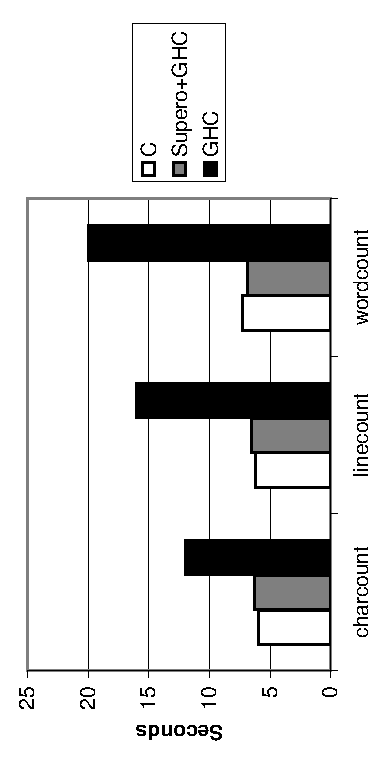
\includegraphics[scale=0.75,angle=270]{supero-wc.eps}
\end{center}
\caption{Benchmarks with C, Supero+GHC and GHC alone.}
\label{fig:c_results}
\end{figure}

The results are given in Figure \ref{fig:c_results}. In all the benchmarks C and Supero are within 10\% of each other, while GHC trails further behind.

\subsection{Identified Haskell Speedups}

During initial trials using these benchmarks, we identified two unnecessary bottlenecks in the Haskell version of word counting. Both were remedied before the presented results were obtained.

\paragraph{Slow \textsf{isSpace} function}

The first issue is that |isSpace| in Haskell is much more expensive than |isspace| in C. The simplest solution is to use a FFI (Foreign Function Interface) \cite{spj:awkward_squad} call to the C |isspace| function in all cases, removing this factor from the benchmark. A GHC bug (number 1473) has been filed about the slow performance of |isSpace|.

\begin{figure}
\begin{code}
words :: String -> [String]
words s = case  dropWhile isSpace s of
                []  ->  []
                x   ->  w : words y
                        where (w, y) = break isSpace x

words' s = case  dropWhile isSpace s of
                 []    ->  []
                 x:xs  ->  (x:w) : words' (drop1 z)
                           where (w, z) = break isSpace xs

drop1 []      = []
drop1 (x:xs)  = xs
\end{code}
\caption{The |words| function from the Haskell standard libraries, and an improved |words'|.}
\label{fig:words}
\end{figure}

\paragraph{Inefficient \textsf{words} function}

The second issue is that the standard definition of the |words| function (given in Figure \ref{fig:words}) performs two additional |isSpace| tests per word. By appealing to the definitions of |dropWhile| and |break| it is possible to show that in |words| the first character of |x| is not a space, and that if |y| is non-empty then the first character is a space. The revised |words'| function uses these facts to avoid the redundant |isSpace| tests.

\subsection{Potential GHC Speedups}

% NOTE: Shorten this section if space needed

We have identified three factors limiting the performance of residual programs when compiled by GHC. These problems cannot be solved at the level of Core transformations. We suspect that by fixing these problems, the Supero execution time would improve by between 5\% and 15\%.

\paragraph{Strictness inference}

The GHC compiler is overly conservative when determining strictness for functions which use the FFI (GHC bug 1592). The |getchar| function is treated as though it may raise an exception, and terminate the program, so strict arguments are not determined to be strict. If GHC provided some way to mark an FFI function as not generating exceptions, this problem could be solved. The lack of strictness information means that in the line and word counting programs, every time the accumulator is incremented, the number is first unboxed and then reboxed \cite{spj:unboxing}.

\paragraph{Heap checks}

The GHC compiler follows the standard STG machine \cite{spj:stg} design, and inserts heap checks before allocating memory. The purpose of a heap check is to ensure that there is sufficient memory on the heap, so that allocation of memory is a cheap operation guaranteed to succeed. GHC also attempts to lift heap checks: if two branches of a case expression both have heap checks, they are replaced with one shared heap check before the case expression. Unfortunately, with lifted heap checks, a tail-recursive function that allocates memory only upon exit can have the heap test executed on every iteration (GHC bug 1498). This problem affects the character counting example, but if the strictness problems were solved, it would apply equally to all the benchmarks.

\paragraph{Stack checks}

The final source of extra computation relative to the C version are stack checks. Before using the stack to store arguments to a function call, a test is performed to check that there is sufficient space on the stack. Unlike the heap checks, it is necessary to analyse a large part of the flow of control to determine when these checks are unnecessary. It is not clear how to reduce stack checks in GHC.

\subsection{Why Supero Outperforms C for the Wordcount Benchmark}

The most curious result is that Supero outperforms C on wordcounting, by about 6\% -- even with the problems discussed! The C program presented in Figure \ref{fig:c_words} is not optimal. The variable \verb"last_space" is a boolean, indicating whether the previous character was a space, or not. Each time round the loop a test is performed on \verb"last_space", even though its value was determined and tested on the previous iteration. The way to optimise this code is to have two specialised variants of the loop, one for when \verb"last_space" is true, and one for when it is false. When the value of \verb"last_space" changes, the program would transition to the other loop. This pattern effectively encodes the boolean variable in the program counter, and is what the Haskell program has managed to generate from the high-level code.

However, in C it is quite challenging to capture the required control flow. The program needs two loops, where both loops can transition to the other. Using \texttt{goto} turns off many critical optimisations in the C compiler. Tail recursion is neither required by the C standard, nor supported by most compilers. The only way to express the necessary pattern is using nested while loops, but unlike newer imperative languages such as Java, C does not have named loops -- so the inner loop cannot break from the outer loop if it reaches the end of the file. The only solution is to place the nested while loops in a function, and use \texttt{return} to break from the inner loop. This solution would not scale to a three-valued control structure, and substantially increases the complexity of the code.

\section{Performance Compared With GHC Alone}
\label{sec:haskell_results}

The standard set of Haskell benchmarks is the nofib suite \cite{nofib}. It is divided into three categories of increasing size: imaginary, spectral and real. Even small Haskell programs increase in size substantially once libraries are included, so we have limited our attention to the benchmarks in the imaginary section. All benchmarks were run with parameters that require runtimes of between 3 and 5 seconds for GHC.

We exclude two benchmarks, paraffins and gen\_regexps. The paraffins benchmark makes substantial use of arrays, and we have not yet mapped the array primitives of Yhc onto those of GHC, which is necessary to run the transformed result. The gen\_regexps benchmark tests character processing: for some reason (as yet unknown) the supercompiled executable fails.

\begin{figure}
\begin{center}
% http://csdl.ics.hawaii.edu/FAQ/chart-ps.html
\includegraphics[scale=0.75,angle=270]{supero-nofib.eps}
\end{center}
\vspace{-4mm}

\textbf{Supero} uses the $\bowtie$ generalisation method; \textbf{msg} uses the msg function for generalisation; \textbf{spine} applies no generalisation operation; \textbf{none} never performs any inlining.

\vspace{2mm}
\caption{Runtime, relative to GHC being 1.}
\label{fig:haskell_results}
\end{figure}

\begin{table}

\begin{tabular}{lrrrrrr}
\textbf{Program} & \hspace{5mm}\textbf{Supero} & \hspace{5mm}\textbf{msg} & \hspace{5mm}\textbf{spine} & \hspace{5mm}\textbf{none} & \hspace{5mm}\textbf{Size} & \hspace{5mm}\textbf{Memory} \\
bernouilli 		& 1.41 & 1.53 & 1.58 & 1.18 & 1.10 & 0.97 \\
digits-of-e1	& 1.03 & 1.16 & 1.03 & 1.06 & 1.01 & 1.11 \\
digits-of-e2	& 0.72 & 0.72 & 0.72 & 1.86 & 1.00 & 0.84 \\
exp3\_8			& 1.00 & 1.00 & 1.00 & 1.01 & 0.99 & 1.00 \\
integrate 		& 0.46 & 0.47 & 0.46 & 4.01 & 1.02 & 0.08 \\
primes 			& 0.57 & 0.57 & 0.88 & 0.96 & 1.00 & 0.98 \\
queens 			& 0.79 & 0.96 & 0.83 & 1.21 & 1.01 & 0.85 \\
rfib 			& 0.97 & 0.97 & 0.97 & 1.00 & 1.00 & 1.08 \\
tak 			& 0.72 & 1.39 & 1.39 & 1.39 & 1.00 & 1.00 \\
wheel-sieve1 	& 0.98 & 1.11 & 1.42 & 5.23 & 1.19 & 2.79 \\
wheel-sieve2 	& 0.87 & 0.63 & 0.89 & 0.63 & 1.49 & 2.30 \\
x2n1 			& 0.58 & 0.64 & 1.61 & 3.04 & 1.09 & 0.33 \\
\end{tabular}
\vspace{2mm}

\textbf{Program} is the name of the program; \textbf{Supero} uses the $\bowtie$ generalisation method; \textbf{msg} uses the msg function for generalisation; \textbf{spine} applies no generalisation operation; \textbf{none} never performs any inlining; \textbf{Size} is the size of the Supero generated executable; \textbf{Memory} is the amount of memory allocated on the heap by the Supero executable.

\vspace{4mm}
\hrule
\vspace{2mm}
\caption{Runtime, relative to GHC being 1.}
\label{tab:haskell_results}
\end{table}

The results of these benchmarks are given in Figure \ref{fig:haskell_results}, along with detailed breakdowns in Table \ref{tab:haskell_results}. All results are relative to the runtime of a program compiled with GHC -O2, lower numbers being better. The first three variants (Supero, msg, spine) all use homeomorphic embedding as the termination criterion, and $\bowtie$, msg or nothing respectively as the generalisation function. The final variant, none, uses a termination test that always causes a residuation. The `none' variant is useful as a control to determine which improvements are due to bringing all definitions into one module scope, and which are a result of supercompilation. Compilation times ranged from a few seconds to five minutes.

The Bernouilli benchmark is the only one where Supero is slower than GHC by more than 3\%. The reason for this anomaly is that a dictionary is referred to in an inner loop which is specialised away by GHC, but not by Supero.

With the exception of the wheel-sieve2 benchmark, our $\bowtie$ generalisation strategy performs as well as, or better than, the alternatives. While the msg generalisation performs better than the empty generalisation on average, the difference is not as dramatic.

\subsection{GHC's optimisations}

For these benchmarks it is important to clarify which optimisations are performed by GHC, and which are performed by Supero. The `none' results show that, on average, taking the Core output from Yhc and compiling with GHC does \textit{not} perform as well as the original program compiled using GHC. GHC has two special optimisations that work in a restricted number of cases, but which Supero produced Core is unable to take advantage of.

\paragraph{Dictionary Removal} Functions which make use of type classes are given an additional dictionary argument. In practice, GHC specialises many such functions by creating code with a particular dictionary frozen in. This optimisation is specific to type classes -- a tuple of higher order functions is not similarly specialised. After compilation with Yhc, the type classes have already been converted to tuples, so Supero must be able to remove the dictionaries itself. One benchmark where dictionary removal is critical is digits-of-e2.

\paragraph{List Fusion} GHC relies on names of functions, particularly |foldr|/|build| \cite{spj:rules}, to apply special optimisation rules such as list fusion. Many of GHC's library functions, for example |iterate|, are defined in terms of |foldr| to take advantage of these special properties. After transformation with Yhc, these names are destroyed, so no rule based optimisation can be performed. One example where list fusion is critical is primes, although it occurs in most of the benchmarks to some extent.

\begin{comment}
\subsection{Termination Bound}
\label{sec:results_bound}

Table \ref{tab:haskell_results} includes a column indicating the size bound that was applied to expressions. Out of the five benchmarks, both primes and queens could be run at any greater bound and would still produce the same program -- the direct repetition criteria (see \S\ref{sec:direct}) bounds the expressions on its own. For the remaining programs, a bound was chosen to ensure that the compilation process was quick (under two seconds). By increasing the termination bound the size of the residual program would increase, but the generated program may execute faster.

The existence of a termination bound requiring different values for different programs is a cause for concern. In a large program it is likely that different parts of the program would require different bounds on the size of the generated expression -- something not currently possible. We suspect that the most promising direction is to augment the direct repetition criterion to obtain termination in all practical cases without resorting to a depth bound.
\end{comment}

\section{Related Work}
\label{sec:related}

Supercompilation \cite{supercompilation,turchin:experiments} was introduced by Turchin for the Refal language \cite{refal}. Since this original work, there have been various suggestions of both termination strategies and generalisation strategies \cite{turchin:generalisation,sorensen:supercompilation,leuschel:homeomorphic}. The original supercompiler maintained both positive and negative knowledge, but our implementation is a simplified version maintaining only positive information \cite{secher:perfect_supercompilation}.

The issue of let expressions in supercompilation has not previously been a primary focus. If lets are mentioned, the usual strategy is to substitute all linear lets and residuate all others. Lets have been considered in a strict setting \cite{jonsson:supercompilation}, where they are used to preserve termination semantics, but in this work all strict lets are inlined without regard to loss of sharing. Movement of lets can have a dramatic impact on performance: carefully designed let-shifting transformations give an average speedup of 15\% in GHC \cite{spj:letfloating}, suggesting let expressions are critical to the performance of real programs.

\paragraph{Partial evaluation} There has been a lot of work on partial evaluation \cite{jones:partial_evaluation}, where a program is specialised with respect to some static data. The emphasis is on determining which variables can be entirely computed at compile time, and which must remain in the residual program. Partial evaluation is particularly appropriate for specialising an interpreter with an expression tree to generate a compiler automatically, often with an order of magnitude speedup, known as the First Futamura Projection \cite{futanama:projections}. Partial evaluation is not usually able to remove intermediate data structures. Our method is certainly less appropriate for specialising an interpreter, but in the absence of static data, is still able to show improvements.

% Partial evaluation has been applied to full-scale functional languages, such as Curry
% \cite{albert:partial_evaluation_curry}.

\paragraph{Deforestation} The deforestation technique \cite{wadler:deforestation} removes intermediate lists in computations. This technique has been extended in many ways to encompass higher order deforestation \cite{marlow:higher_order_deforestation} and work on other data types \cite{coutts:string_fusion}. Probably the most practically motivated work has come from those attempting to restrict deforestation, in particular shortcut deforestation \cite{gill:shortcut_deforestation}, and newer approaches such as stream fusion \cite{coutts:stream_fusion}. In this work certain named functions are automatically fused together. By rewriting library functions in terms of these special functions, fusion occurs.

\paragraph{Whole Program Compilation} The GRIN approach \cite{grin} uses whole program compilation for Haskell. It is currently being implemented in the jhc compiler \cite{jhc}, with promising initial results. GRIN works by first removing all functional values, turning them into case expressions, allowing subsequent optimisations. The intermediate language for jhc is at a much lower level than our Core language, so jhc is able to perform detailed optimisations that we are unable to express.

\paragraph{Lower Level Optimisations} Our optimisation works at the Core level, but even once efficient Core has been generated there is still some work before efficient machine code can be produced. Key optimisations include strictness analysis and unboxing \cite{spj:unboxing}. In GHC both of these optimisations are done at the Core level, using a Core language extended with unboxed types. After this lower level Core has been generated, it is then compiled to STG machine instructions \cite{spj:stg}, from which assembly code is generated. There is still work being done to modify the lowest levels to take advantage of the current generation of microprocessors \cite{marlow:pointer_tagging}. We rely on GHC to perform all these optimisations after Supero generates a residual program.

\begin{comment}
\paragraph{Other Transformations} One of the central operations within our optimisation in inlining, a technique that has been used extensively within GHC \cite{spj:inlining}. We generalise the constructor specialisation technique \cite{spj:specconstr}, by allowing specialisation on any arbitrary expression, including constructors.

One optimisation we do not currently support is the use of user provided transformation rules \cite{spj:rules}, which can be used to automatically replace certain expressions with others -- for example |sort . nub| removes duplicates then sorts a list, but can be done asymptotically faster in a single operation.
\end{comment}

\section{Conclusions and Future Work}
\label{sec:conclusion}

Our supercompiler is simple -- the Core transformation is expressed in just 300 lines of Haskell. Yet it replicates many of the performance enhancements of GHC in a more general way. We have modified some of the techniques from supercompilation, particularly with respect to let bindings and generalisation. Our initial results are promising, but incomplete. Using our supercompiler in conjunction with GHC we obtain an average runtime improvement of 16\% for the imaginary section of the nofib suite. To quote Simon Peyton Jones, ``an average runtime improvement of 10\%, against the baseline of an already well-optimised compiler, is an excellent result'' \cite{spj:specconstr}.

There are three main areas for future work:

\begin{description}
\item[More Benchmarks] The fifteen benchmarks presented in this paper are not enough. We would like to obtain results for larger programs, including all the remaining benchmarks in the nofib suite.
\item[Runtime Performance] Earlier versions of Supero \cite{me:supero_ifl} managed to obtain substantial speed ups on benchmarks such as exp3\_8. The Bernouilli benchmark is currently problematic. There is still scope for improvement.
\item[Compilation Speed] The compilation times are tolerable for benchmarking and a final optimised release, but not for general use. Basic profiling shows that over 90\% of supercompilation time is spent testing for a homeomorphic embedding, which is currently done in a na\"{i}ve manner -- dramatic speedups should be possible.
\end{description}

The Programming Language Shootout\footnote{\url{http://shootout.alioth.debian.org/}} has shown that low-level Haskell can compete with low-level imperative languages such as C. Our goal is that Haskell programs can be written in a high-level declarative style, yet still perform competitively.



%include thesis.fmt

\chapter{First-Order Reduction}

This chapter deals with the reduction from a higher-order Core language to a primarily first-order Core language. Our motivation is that the Catch analysis tool (see Chapter \ref{chp:catch}) is designed to work only upon a first-order language, but our method may have use for other analysis tools, particularly termination checking \cite{serini:term,someone_else,someone_else}. The transformations presented in this chapter are all semantics preserving, but do \textit{not} all preserve sharing. As such, these transformations may not be suitable for optimisation, but are perfectly acceptable for analysis methods.


\section{Higher-Order Elements}

A program can be said to be higher-order if at runtime the program generates and manipulates functional values. In our Core language as currently defined, the expression |id 1| first evaluates |id| to a functional value, then applies the argument |1|. For our higher-order classification we treat a top-level function symbol and all statically given application arguments as one unit, meaning |id 1| is not a functional value.

\begin{example}
\label{ex:ho_elements}
The following two functions can be thought of as having functional elements:

\begin{code}
even = not . odd

map f x = case  x of
                []    -> []
                y:ys  -> f y : map f ys
\end{code}

The |even| function passes |not| and |odd| to the function |(.)|, both of which are functional values. In addition, the |(.)| function, when applied to only two arguments, returns a functional value. The definition of |map| does not create any functional values, but applies the variable |f| to an argument, suggesting that |f| is a functional value.
\end{example}

We classify higher-order elements as either \textit{creating} or \textit{applying} functional values.


\subsection{Creating Functional Values}

The most obvious way to create a functional value in our Core language is with an explicit lambda expression. The other way is to \textit{curry} or \textit{partially apply} a function, by passing fewer arguments than the arity of the function.

\begin{example}
\begin{code}
example1 = (\x -> x) 42

example2 xs = map id xs
\end{code}

Here |example1| contains an explicit lambda, which is a functional value. In |example2| the function |id| has an arity of 1, but is not given any arguments, and hence is a functional value.
\end{example}

It is possible for a program to have either one of these syntatic conditions, but at runtime, not create any functional values. Consider the following code:

\begin{code}
main = case  True of
             True   -> 1
             False  -> (\x -> x) 2
\end{code}

Here the |True| branch will always be taken due to the known case scrutinee. The |False| branch would create a functional value if taken, but as it will never be taken, this program will never create a functional value. This situation can be thought of as having functional elements in dead code.


\subsection{Applying Functional Values}

There are two ways to make use of functional values. The first is to apply an argument to an expression which is not a constructor or a top-level function. The second is to give a function more arguments than its associated arity.

\begin{example}
\begin{code}
example1 f = f 42

example2 = even 42
\end{code}

In |example1| the argument |f| is applied to the value 42, suggesting that |f| is functional. In |example2|, |even| is applied to one argument. Using the definition of |even| from Example \ref{ex:ho_elements}, with arity 0, this causes |even| to be given more arguments than its arity.
\end{example}

As before, we can construct an example where a functional value is applied, but which never occurs at runtime due to dead code. Another way of constructing an apparent application of a functional value is using |undefined| or a call to |error|.

\begin{example}
\begin{code}
main = error "bang" 42
\end{code}

Here the |error| primitive is being given two arguments, even though at first glance it appears to only take one. The is possible because the type of error is |String -> alpha|, where |alpha| is completely unconstrained and can be anything, including a functional type.
\end{example}


\subsection{First-Order Core}

We define a program to be first-order if it contains no expressions of the two types identified as creating functional values. In order to allow the property to be calculated statically, we ignore the issue of dead code.

There exist programs, or fragments of code, which cannot be reduced to first-order. We present several examples in turn, explaining why a first-order reduction is not possible.

\begin{example}
\begin{code}
main = [id]
\end{code}

In this example, the |main| function returns a functional value inside a constructor. We cannot remove the functional value without changing the semantics of the |main| function, which is called from outside the our program, and hence cannot be altered. A related situation is:

\begin{code}
main = id
\end{code}

Here we can only reduce this program to first-order if we are allowed to increase the arity of |main| from zero to one. This situation occurs frequently in Haskell programs, whose |main| definition is typically of type |IO ()|. In the Yhc compiler, used to generate our Core language, the definition of |IO| is:

\begin{code}
newtype IO alpha = IO (World -> _E alpha)
\end{code}

At compilation time the |newtype| wrapper is removed, leaving a function from |World| to |_E alpha|. The |main| argument therefore takes a |World| parameter, before returning a first-order result. We permit the increasing of the arity of |main|.
\end{example}

\begin{example}
\begin{code}
main = id `seq` 42
\end{code}

Here a functional value (|id|) is passed to the primitive |seq|. As we are not able to peer inside the primitive, and must preserve its interface, we cannot remove this functional value. For most primitives, such as arithmetic operations, the types ensure that no functional values are passed as arguments. However, the |seq| primitive is of type |alpha -> beta -> beta|, allowing any type to be passed as either of the arguments, including functional values.

Another primitive which permits functional values is |primCatch :: alpha -> (beta -> alpha) -> alpha|. While |seq| merely permits functional values, |primCatch| actually \textit{requires} that the second argument is a functional value.
\end{example}

In both these examples, a functional value must be created as it is required by either the interface to a primitive, or the interface to the root function. In a similar manner, the root function may have a functional argument, or a primitive may return a functional value, resulting in a functional application.

If neither of the above cases occurs, then it is always possible to remove all function values from a Core program. One method for removing higher-order functions is Reynolds style defunctionalisation, which we detail first. Next we detail our method, which has some important differences from Reynold's method.


\section{Reynolds style defunctionalization}

Reynolds style defunctionalization \cite{reynolds:defunc} is the seminal method for generating a first-order equivalent of a higher-order program.

\begin{example}
\begin{code}
map f x = case  x of
                []      -> []
                (y:ys)  -> f y : map f ys
\end{code}

\noindent Defunctionalization works by creating a data type to represent all values that |f| may take anywhere in the whole program. For instance, it might be:

\ignore\begin{code}
data Function = Head | Tail

apply Head  x = head  x
apply Tail  x = tail  x

map f x = case  x of
                []    -> []
                y:ys  -> apply f a : map f as
\end{code}

\noindent Now all calls to |map head| are replaced by |map Head|.
\end{example}

This method naturally extends to partial application. To take a more complicated example, where higher-order functions are being used to store information:

\begin{example}
\begin{code}
type Map = String -> Int

new :: Map
new _ = 0

get :: String -> Map -> Int
get key mp = mp key

add :: String -> Int -> Map -> Map
add key val mp s = if s == key then val else get key mp

test = get "foo" (add "bar" 4 (add "baz" 2 new))
\end{code}

\noindent The above code creates a functional map, which uses a higher-order function to store a mapping from |String| to |Int|. The |add| function inserts a new key/value pair into the map. This is transformed with defunctionalization to:

\begin{code}
data Function  =  New
               |  Add3 String Int Function

apply  New                 x = new x
apply  (Add3 y_1 y_2 y_3)  x = add y_1 y_2 y_3 x

new _ = 0

get key mp = apply mp key

add key val mp s = if s == key then val else get key mp

test = get "foo" (Add3 "bar" 4 (Add3 "baz" 2 New))
\end{code}

Here we use the constructor |Add3| to represent the |add| function with three arguments pre-applied. Note that the |Function| data type now serves to store a linked-list of the values with |New| serving a similar role to |[]|, and |Add3| storing one key/value pair along with the remainder of the list.
\end{example}

Defunctionalized code is still type safe, but type checking would require a dependently typed language. The method is complete, removing all possible higher-order functions, and preserves space behaviour. The disadvantage is that the transformation essentially embeds a mini-interpreter for the original program into the new program. The flow control is complicated by the extra level of indirection.

Some uses of Reynold's method include as preprocessing step in a whole-program analysis \cite{grin,jhc} and as a step in a program transformation \cite{graham_hutton_calculating_an_exceptional_machine}.

\section{Our First-Order Reduction Method}

A natural desire would be to eliminate the higher-order aspects of a program, without introducing any new data structures. However, it is simple to show that this transformation is not possible. Given a program, we can remove all data structures by Church encoding \cite{church_encode}. If we then had a transformation which made the program first-order \textit{without} introducing any data, we would end up with a program without data or closures, which is therefore incapable of storing an unbounded amount of information. Since with higher-order functions we can implement a Turing machine \cite{turing:halting}, and without an unbounded store we cannot, such a transformation cannot exist.

Our reduction method proceeds in four steps, each removing some higher-order elements, without introducing any data structures. Each step is independently terminating, and are combined using a fixed point operator. Because our method terminates and does not introduce any data structures, it is necessarily incomplete -- but Reynold's method can be used afterwards.

Our method proceeds in four steps:

\begin{code}
firstify = lambdas +|+ simplify +|+ inline +|+ specialise
\end{code}

Each stage will be described separately. The overall control of the algorithm is given by the |(+||+)| operate, defined as:

\begin{code}
infixl +|+

(+|+) :: Eq alpha => (alpha -> alpha) -> (alpha -> alpha) -> alpha -> alpha
(+|+) f g x  = fix (fix x . y)

fix :: Eq alpha => (alpha -> alpha) -> alpha -> alpha
fix f x = if x == x2 then x else fix f x2
    where x2 = f x
\end{code}

The |(+||+)| operator applies the first argument until it reaches a fixed point, then applies the second argument. If the second argument changes the value, the first argument is tried again until a fixed point is achieved. This formulation has several important properties:

\begin{description}
\item[Idempotent in each function] After the operation has completed, applying either |f| or |g| will not change the value.

\begin{code}
forall f g x `o` let r = (+|+) f g x in f r == r && g r == r
\end{code}

\item[Idempotent] The operation as a whole is idempotent.

\begin{code}
forall f g x `o` let r = (+|+) f g x in r == (+|+) f g r
\end{code}

\item[Function ordering] The function |f| will have reached a fixed point before the function |g| is applied.
\end{description}

The final property allows us to overlap the application sites between the two arguments, but guarantee the first will always be chosen. The other two properties ensure that when the operation finishes there will be no further sites where application could occur.

The operator is left associative, meaning that the code can be rewritten with explicit bracketing as:

\begin{code}
firstify = ((lambdas +|+ simplify) +|+ inline) +|+ specialise
\end{code}

Within this chain we guarantee that the end result will be idempotent with respect to any of the functions, and before any function is invoked, all those to the left of it will be idempotent.

The operator |(+||+)| is written for clarity, not for speed. If the first argument is idempotent on its own, then additional unnecessary work is performed. In the case of chaining operators, the left function is guaranteed to be idempotent in all but the first case, so much computation is duplicated. The |(+||+)| operator also checks for global equality, when typically operations will only operate within some locality, which could be exploited.

We now describe each of the stages in the algorithm separately.

\subsection{Lambda Insertion (|lambdas|)}

The first stage removes all occurrences of partial application, replacing them with explicit lambda expressions.

\begin{examplerevisit}{\ref{ex:ho_elements}}
\begin{code}
even = \x -> (.) (\y -> not y) (z -> odd z) x
\end{code}

Here the |even| function, which previously had three instances of partial application, has three lambda expressions inserted. Now each function is applied to a number of arguments equal to its arity. In this particular instance, the introduction of lambda expressions changes the arity of |even| from 0 to 1, possibly requiring applications of |even| to become partially applied.
\end{examplerevisit}

For each partially applied function, a lambda expression is inserted to ensure that the function is now given at least as many arguments as its associated arity. This step trades one form of function creation for another form, but has the advantage of making functional values more explicit.

\subsection{Simplification (|simplify|)}

\begin{figure}
\renewcommand{\f}[2]{\vspace{-7mm} #2 & (#1) \\}

\begin{flushright}
\begin{tabular}{p{8cm}r}
\f{case-lam}{
\begin{code}
case x of {... ; c vs_ -> \v -> y ; ...}
    => \v' -> case x of {... ; c vs_ -> \v -> y ; ...} v'
\end{code}}

\f{bind-lam}{
\begin{code}
let v = \v' -> x in y
    => y[v/ \v' -> x]
\end{code}}


\f{let-lam}{
\begin{code}
let v = x in \v' -> y
    => \v' -> let v = x in y
\end{code}}
\end{tabular}
\end{flushright}
\caption{Lambda Simplification rules.}
\label{fig:lambda_simplify}
\end{figure}

The second stage attempts to move lambda's upwards until they form part of the arity of a function. This stage makes use of the general simplification rules (Figure \ref{fig:simplify}), along with some additional rules which deal with lambda expressions, given in Figure \ref{fig:lambda_simplify}.

The rule (case-lam) lifts a lambda out from within a case alternative to outside the case value. The (bind-lam) rule inlines a lambda bound in a let expression. The (let-lam) rule is the one responsible for the largest loss of sharing, promoting a lambda expression outside a let.

\begin{example}
\begin{code}
f x = let i = expensive x
      in \j -> i + j

main xs = map (f 1) xs
\end{code}

In the above example, |expensive 1| is computed once and saved. Every application of the functional argument within |map| performs a single |(+)| operation. After applying the (let-lam) rule we get:

\begin{code}
f x j = let i = expensive x
        in i + j
\end{code}

Now |expensive| will be recomputed for every element in |xs| -- potentially a very severe speed penalty.
\end{example}

The loss of sharing is not purely theoretical, the Uniplate library makes use of a let within a lambda (see \S\ref{sec:optimise_playdata}) to keep a scoreboard. The (let-lam) rule would make the scoreboard mechanism a severe performance penalty.

\subsection{Inlining (|inline|)}

After inserting additional lambda expressions, and performing simplification, there may still be residual lambda expressions which are not at the top level of a function. The simplification rules will promote lambda expressions up above let expressions and case expressions. With the additional rules, the only residual lambda expressions will be as arguments to either a constructor, or a function. The inline stage deals with lambda expressions which are residual to a constructor at the top level, the specialise stage deals with all remaining lambda expressions.

\begin{example}
Given a program making use of type class dictionaries, as detailed in \S\ref{sec:dictionary_transformation}, we may end up with the following code:

\begin{code}
eqInt = (\x y -> primEqInt x y, \x y -> primNeqInt x y)
(==) d x y = d x y

main = (==) eqInt 1 2
\end{code}

Here the lambda expression including |primEqInt| is an argument to the constructor |(,)| in the top-level of |eqInt|. The inline stage will inline the |eqInt| function anywhere it occurs, resulting in:

\begin{code}
(==) (a,b) x y = a x y

main = (==) (\x y -> primEqInt x y, \x y -> primNeqInt x y) 1 2
\end{code}

The lambda expressions are still present, but hopefully can be removed using other techniques.
\end{example}

The general rule is to inline all functions containing a subexpression |alpha|, where: |alpha| is a constructor application with one argument which is a lambda expression; and |alpha| is not a subexpression of any argument to a function application.

\begin{example}
\begin{code}
yes0 = [\x -> x]
yes1 = Maybe [\x -> x]
yes2 = let y = 1 in [\x -> x]
no0 = \x -> id x
no1 = [id (\x -> x)]
no2 = id [\x -> x]
\end{code}

In this example, we would inline the |yes| functions, but none of the others. In |no0| there is no constructor, so the first condition does not apply. In |no1| there is a constructor, but the lambda expression is not an argument to the constructor. In |no2| there is a lambda expression as an argument to a constructor, but that subexpression is an argument to a function application.
\end{example}

The |inline| rule deals with situations where functions evaluate to a data structure containing functional values. This situation occurs regularly with the standard dictionary implementation, but rarely in other situations. The inline rule does not actually remove functional values, but can bring their use and creation closer together, and thus helps them be removed.


\subsection{Specialisation (|special|)}

The original Catch tool \cite{me:catch_tfp} uses specialisation to remove higher-order functions. For each application of a function to functional arguments, a specialised variant is created, and used where applicable. The process follows the same pattern as constructor specialisation \cite{spj:specconstr}, but applied where function arguments are partially applied functions, rather than known constructors. Examples of common functions whose applications can usually be made first-order include |map|, |filter|, |foldr| and |foldl|.

The specialisation transformation makes use of \textit{templates}. A template is an expression where some sub-expressions are omitted, denoted by an underscore. The process of specialisation proceeds as follows:

\begin{enumerate}
\item Find all functions which have functional arguments, and generate templates, omitting first-order components.
\item For each template, generate an associated function, specialised to the template.
\item For each subexpression matching a template, replace it with the associated function.
\end{enumerate}

\begin{example}
\begin{code}
main xs = map (\x -> x) xs

map f xs = case  xs of
                 []    -> []
                 y:ys  -> f y : map f ys
\end{code}

The specialisation first finds the application of |map| within |main|, and generates the template |map (\x -> x) _| -- omitting the |xs| which is not obviously a functional value. It then generates the name |map_id| for the template, and generates an appropriate function body. Next all calls matching the template are replaced with calls to |map_id|, including in the call to |map| within the freshly generated |map_id|.

\begin{code}
main xs = map_id xs

map_id xs = case  xs of
                  []    -> []
                  y:ys  -> y : map_id ys
\end{code}

The resulting code has no functional values within it.
\end{example}

\subsubsection{Generating Templates}

A template is generated if an expression is an application to a top-level function, whose arguments include a sub-expression which is a lambda expression. The template includes all sub-expressions whose removal would lead to higher-order elements, or which have free variables from a bound variable.

\begin{example}
\begin{code}
id (\x -> x)              => id (\x -> x)
id (Maybe (\x -> x))      => id (Maybe (\x -> x))
id (Maybe (\x -> x + 3))  => id (Maybe (\x -> x + _))
id (Maybe (\x -> x + y))  => id (Maybe (\x -> x + _))
\end{code}

In all three examples, the |id| function has an argument which has a lambda expression as a subexpression. In the final two cases, the |3| and |y| are not dependent on variables bound within the lambda, and are left as unspecified.  The |Maybe| and |+| functions are also not dependent on the bound variables, however their removal would require a functional argument as a parameter, so are left as part of the template.
\end{example}

\subsubsection{Generating Functions}

Given a template, to generate an associated function, a unique function name is allocated to the template. Each |_| within the template is assigned a free variable, as an argument to the new function, then the body is produced by unfolding the outer function symbol in the template once.

\begin{example}
\label{ex:map_id}
Following the |map (\x -> x) _| template from above, we can generate |v_1| as the unique free variable for the single |_| placeholder, and |map_id| as the function name:

\begin{code}
map_id v_1 = map (\x -> x) v_1
\end{code}

In the next step, we unfold the definition of map once:

\begin{code}
map_id v_1 = let  f   = \x -> x
                  xs  = v_1
             in   case  xs of
                        []    -> []
                        y:ys  -> f y : map f ys
\end{code}

Now the generation of the specialised variant is complete. To give an idea of how the final function is calculated, after the simplification rules introduced in Figure \ref{fig:lambda_simplify}, we end up with:

\begin{code}
map_id v_1 =  let  xs = v_1
              in   case  xs of
                         []    -> []
                         y:ys  -> y : map (\x -> x) ys
\end{code}
\end{example}

\subsubsection{Using Templates}

After a function has been generated for each template, every expression matching a template can be replaced by a call to the new function. Every subexpression corresponding to an undecided element is passed as an argument. Continuing with the generated code from Example \ref{ex:map_id}, we end up with:

\begin{code}
map_id v_1 =  let  xs = v_1
              in   case  xs of
                         []    -> []
                         y:ys  -> y : map_id ys
\end{code}

We have now eliminated all the functional values from within this operation.


\section{Proof of Correctness}


\section{Proof of Termination}



\subsection{Termination of Inlining}

As with specialisation, the inlining of functions until a fixed point can give rise to non-termination:

\begin{example}
\begin{code}
f = if condition then f else id
\end{code}

The expression bound to |f| will repeatedly grow in size as inlining is applied, and will remain unsaturated. We stop this problem by inlining a function at all application sites, but only once. In this example we would end up with:

\begin{code}
f = if condition then (if condition then f else id) else id
\end{code}

At this stage we have inlined |f| once, so do not inline |f| again.
\end{example}

\subsection{Termination of Specialisation}

A natural extension of specialisation is to take the fixed point, eliminating unsaturated expressions in generated functions. Unfortunately, such an algorithm would not terminate.

\begin{example}
\begin{code}
data Wrap a  =  Wrap (Wrap a)
             |  Value a

f x = f (Wrap x)
main = f (Value head)
\end{code}

In the first iteration, this would generate a version of |f| specialised to |Value head|. In the second iteration it would specialise |f| with respect to |Wrap (Value head)|, then in the third with |Wrap (Wrap (Value head))|. We would generate an infinite number of specialisations of |f|.
\end{example}

One simple way to prevent such non-termination is to have a bound on the number of specialisations. Another approach is to use a homeomorphic embedding. All functions relate to some original expression in the Core language, if the expression to be generated was a homeomorphic embedding of an already specialised expression, we can stop.

Using homeomorphic embedding on the previous example, we would generate the following specialised variants of |f (Value head)| and |f (Wrap (Value head))|. Upon attempting to generate the specialised variant |f (Wrap (Wrap (Value head)))| we would abort, with an embedding of |f (Wrap (Value head))|.





\section{Results}

Our preferred method for higher-order function removal is to apply specialisation and inlining interleaved. We have tried our method on the nofib suite, and have the following results.


\chapter{Pattern Match Analysis}


%include paper.fmt

\hsdef{uniplate,descend}

\chapter{Conclusions}
\label{chp:conclusions}

In this thesis we have presented a boilerplate reduction library (Uniplate), an optimiser (Supero), a defunctionalisation method (Firstify) and an analysis tool (Catch), all for the Haskell language. In this chapter we first describe some of the high-level contributions we have made in \S\ref{secE:contributions}, give areas for future work in \S\ref{secE:future_work}, then summarise our approach in \S\ref{secE:the_end}.


\section{Contributions}
\label{secE:contributions}

Specific technical contributions have been given in each chapter. In this section we instead focus on the higher-level contributions -- the overall results that are of benefit to functional programmers.

\subsection{Shorter Programs}

Some of our work enables programmers to write shorter programs. In particular the Uniplate library defines a small set of operations to perform queries and transformations. We have illustrated by example that the boilerplate required in our system is less than in other systems (\S\ref{secU:results_boilerplate}).

\subsection{Faster Programs}

Some of our work helps programs execute faster. Using Supero in conjunction with GHC we obtain an average runtime improvement of 16\% for the imaginary section of the nofib suite. To quote Simon Peyton Jones, ``an average runtime improvement of 10\%, against the baseline of an already well-optimised compiler, is an excellent result'' \cite{spj:specconstr}. The Programming Language Shootout\footnote{\url{http://shootout.alioth.debian.org/}} has shown that low-level Haskell can compete with low-level imperative languages such as C. We hope that our optimiser will allow programs to be written in a high-level declarative style, yet still perform competitively.

We have also invested effort in optimising the Uniplate library. As a result we can express concise traversals without sacrificing speed (\S\ref{secU:results_speed}). In particular, we show a substantial speed up over the SYB library \cite{lammel:syb}.

We developed the Firstify tool for analysis, not performance. However, for many simple examples, the resultant program performs better than the original. If we restricted rules that reduce sharing, our defunctionalisation method may be appropriate for integration into an optimising compiler.

\subsection{Safer Programs}

The Catch tool allows programs to have non-exhaustive patterns, yet still have verifiable pattern-match safety. In practical use the Catch tool has found real bugs in real programs, which have subsequently been fixed (see \S\ref{secC:hscolour}). The XMonad developers found that using the Catch tool encouraged a safer style of programming, paying more attention to partial functions (see \S\ref{secC:xmonad}).

The Uniplate library also encourages a style of programming which can lead to fewer errors. By reducing the volume of code, particularly repetitive code, bugs become easier to spot.

\section{Future Work}
\label{secE:future_work}

\subsection{Robust and Widely Applicable Tools}

We have implemented all the tools described in this thesis. The Uniplate library is already robust and used in real programs. The other tools serve more as prototypes, and have not seen sufficient real-world use to declare them production ready. With the exception of Uniplate, the tools are based around the core language from the Yhc compiler. Currently this core language is generated by the Yhc compiler, as described in \S\ref{secB:generating_core}. Yhc restricts our input programs to the Haskell 98 language. By making use of the GHC front end, we would be able to deal with many language extensions.

Supero, Firstify and Catch all operate on a whole program at a time, requiring sources for all function definitions. This requirement both increases the time required, and precludes the use of closed source libraries. We may be able to relax this requirement, precomputing partial results of libraries, or permitting some components of the program to be ignored. We already supply abstractions of IO functions for Catch, and this mechanism could be extended.

\subsection{Uniplate}

The use of boilerplate reduction strategies in Haskell is not yet ubiquitous, as we feel it should be. The ideas behind the Uniplate library have been used extensively, in projects including the Yhc compiler \citep{me:yhc_core}, the Catch tool, the Reach tool \cite{naylor:reach} and the Reduceron \cite{naylor:reduceron}. In previous versions of Catch there were over 100 Uniplate traversals.

There is scope for further speed improvements: for example, use of continuation passing style may eliminate tuple construction and consumption, and enhanced fusion may be able to eliminate some of the intermediate structures in the |uniplate| function. We have made extensive practical use of the Uniplate library, but there may be other traversals which deserve to be added.

Another area of future work, which others have already begun to explore, is the implementation of Uniplate in other languages. So far, we are aware of versions in ML\footnote{\url{http://mlton.org/cgi-bin/viewsvn.cgi/*checkout*/mltonlib/trunk/com/ssh/generic/unstable/public/value/uniplate.sig}} \cite{ml} and Curry\footnote{\url{http://www.informatik.uni-kiel.de/~pakcs/lib/CDOC/Traversal.html}} \cite{curry}. People have also proposed variations on Uniplate, including merging the Uniplate/Biplate distinction\footnote{\url{http://www-ps.informatik.uni-kiel.de/~sebf/projects/traversal.html}}, and using |descend| as the underlying basis for the library\footnote{\texttt{http://tomschrijvers.blogspot.com/2007/11/\\extension-proposal-for-uniplate.html}}.

\subsection{Supero}

Within Supero, there are three main areas for future work. Firstly, we would like to obtain results for larger programs, including all the remaining benchmarks in the nofib suite. Additional benchmarks will give further insight into the performance benefits that Supero provides.

Secondly, we would like to increase the runtime performance. Earlier versions of Supero \cite{me:supero_ifl} managed to obtain substantial speed ups on benchmarks such as exp3\_8. The Bernouilli benchmark is currently problematic. There is still scope for improvement.

Finally, we would like to increase compilation speed. The compilation times are tolerable for benchmarking and a final optimised release, but not for general use. We have described the major bottlenecks in \S\ref{secS:compile_time}, along with possible strategies for alleviating them.

\subsection{Firstify}

The Firstify library currently meets all the needs of the Catch tool. Within the algorithm, the use of a numeric termination bound in the homeomorphic embedding is regrettable, but practically motivated. We need further research to determine if such a numeric bound is necessary, or if other measures could be used.

\subsection{Catch}

The Catch tool has been applied to a range of benchmarks, and has shown promising results. However, there are obviously safe programs (for example Bernouilli in \S\ref{secC:imaginary}) which cannot be proven safe using MP-constraints. In addition to having insufficient power for some examples, MP-constraints also lack a normal form, requiring simplification rules. While MP-constraints are useful, we suspect there exist better constraint models which still fit into the Catch framework. One option would be to combine constraint models, allowing different constraint models to check different error calls.

The tests so far have not included any particularly large applications, such as the darcs program, a Haskell compiler, or even Catch itself. Further evaluation on large programs would give a better idea of what limits within Catch are most pressing. While we have released the Catch tool, it has not seen much use outside of our evaluation -- end users are likely to have additional requests.

\section{Concluding Remarks}
\label{secE:the_end}

Throughout this thesis we have been motivated by the idea of simplicity. We have attempted to reduce the complexity of our methods, both for implementation and for use. In particular, none of our tools requires any annotations to programs.

The Uniplate library restricts traversals to a uniformly typed value set, allowing the power of well-developed techniques for list processing such as list-comprehensions to be exploited. We feel this decision plays to Haskell's strengths, without being limiting in practice. Hopefully by not requiring complicated language features (particularly `scary' types) we will allow a wider base of users to enjoy the benefits of boilerplate-free programming.

Our supercompiler is simple -- the Core transformation is expressed in just 300 lines of Haskell. Yet it replicates many of the performance enhancements of GHC in a more general way. By simplifying the design, we are able to reduce the unintended interactions between optimisations, a problem that has been referred to as ``swings and roundabouts'' \cite{marlow:fast_curry}.

Many analysis methods, in fields such as strictness analysis and termination analysis, start out first-order and are gradually extended to work on a higher-order language. Defunctionalisation offers an alternative approach: instead of extending the analysis method, we transform the functional values away. The analysis method can remain simple, and still work on all programs.

For the Catch tool we have made two decisions that significantly simplify the design: (1) the target of analysis is a very small, first-order core language; (2) there are finitely many value-set-defining constraints per type. Decision (1) allows for a much simpler analysis method, without the added complexity of higher-order programs. Decision (2) inevitably limits the expressive power of constraints; yet it does not prevent the expression of uniform recursive constraints on the deep structure of values, as in MP-constraints.

Functional programs are well suited to analysis and transformation. In this thesis we have presented a number of techniques, which have been refined in response to practical experiments. We hope that the ideas presented will be of real benefit to functional programmers.


\bibliographystyle{plainnat}
\bibliography

\end{document}
